%
% db3.tex -- daubechies wavelet 3
%
% (c) 2019 Prof Dr Andreas Müller, Hochschule Rapperswil
%
\documentclass[tikz]{standalone}
\usepackage{amsmath}
\usepackage{times}
\usepackage{txfonts}
\usepackage{pgfplots}
\usepackage{csvsimple}
\usetikzlibrary{arrows,intersections,math}
\begin{document}
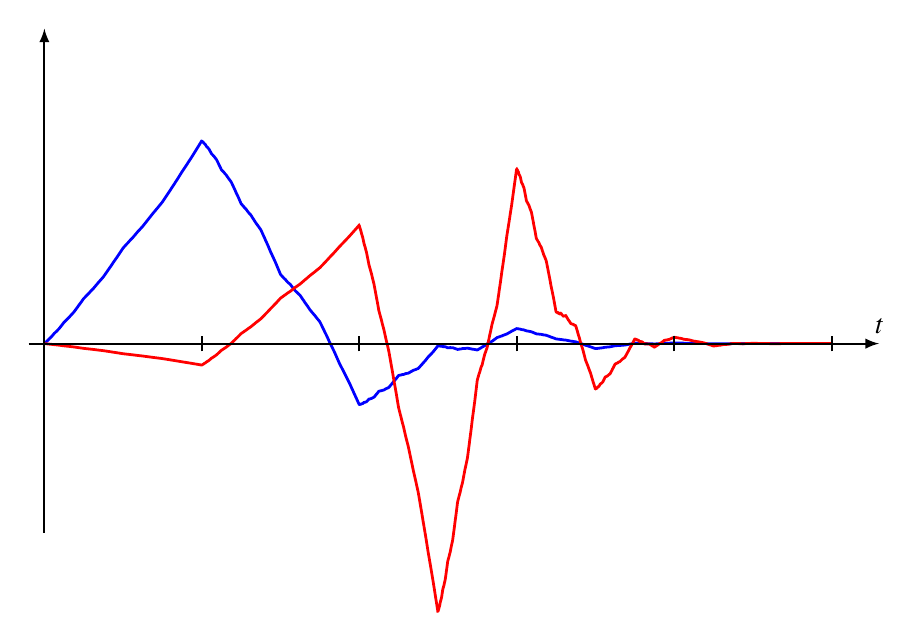
\begin{tikzpicture}[>=latex,scale=2]

\draw[line width=1pt,color=blue] (0.00000, 0.00113)
(0.00195, 0.00274)
--(0.00391, 0.00430)
--(0.00586, 0.00618)
--(0.00781, 0.00780)
--(0.00977, 0.00944)
--(0.01172, 0.01143)
--(0.01367, 0.01355)
--(0.01562, 0.01524)
--(0.01758, 0.01685)
--(0.01953, 0.01863)
--(0.02148, 0.02038)
--(0.02344, 0.02247)
--(0.02539, 0.02471)
--(0.02734, 0.02692)
--(0.02930, 0.02922)
--(0.03125, 0.03103)
--(0.03320, 0.03268)
--(0.03516, 0.03444)
--(0.03711, 0.03613)
--(0.03906, 0.03801)
--(0.04102, 0.03995)
--(0.04297, 0.04180)
--(0.04492, 0.04366)
--(0.04688, 0.04586)
--(0.04883, 0.04820)
--(0.05078, 0.05053)
--(0.05273, 0.05297)
--(0.05469, 0.05530)
--(0.05664, 0.05764)
--(0.05859, 0.06008)
--(0.06055, 0.06256)
--(0.06250, 0.06451)
--(0.06445, 0.06626)
--(0.06641, 0.06807)
--(0.06836, 0.06976)
--(0.07031, 0.07165)
--(0.07227, 0.07357)
--(0.07422, 0.07535)
--(0.07617, 0.07711)
--(0.07812, 0.07911)
--(0.08008, 0.08118)
--(0.08203, 0.08322)
--(0.08398, 0.08530)
--(0.08594, 0.08726)
--(0.08789, 0.08920)
--(0.08984, 0.09118)
--(0.09180, 0.09316)
--(0.09375, 0.09548)
--(0.09570, 0.09794)
--(0.09766, 0.10038)
--(0.09961, 0.10292)
--(0.10156, 0.10538)
--(0.10352, 0.10786)
--(0.10547, 0.11044)
--(0.10742, 0.11307)
--(0.10938, 0.11554)
--(0.11133, 0.11799)
--(0.11328, 0.12048)
--(0.11523, 0.12297)
--(0.11719, 0.12556)
--(0.11914, 0.12819)
--(0.12109, 0.13081)
--(0.12305, 0.13346)
--(0.12500, 0.13556)
--(0.12695, 0.13744)
--(0.12891, 0.13937)
--(0.13086, 0.14116)
--(0.13281, 0.14311)
--(0.13477, 0.14505)
--(0.13672, 0.14685)
--(0.13867, 0.14860)
--(0.14062, 0.15061)
--(0.14258, 0.15268)
--(0.14453, 0.15470)
--(0.14648, 0.15675)
--(0.14844, 0.15865)
--(0.15039, 0.16049)
--(0.15234, 0.16238)
--(0.15430, 0.16424)
--(0.15625, 0.16635)
--(0.15820, 0.16856)
--(0.16016, 0.17073)
--(0.16211, 0.17296)
--(0.16406, 0.17512)
--(0.16602, 0.17727)
--(0.16797, 0.17948)
--(0.16992, 0.18172)
--(0.17188, 0.18381)
--(0.17383, 0.18585)
--(0.17578, 0.18792)
--(0.17773, 0.18996)
--(0.17969, 0.19207)
--(0.18164, 0.19420)
--(0.18359, 0.19630)
--(0.18555, 0.19840)
--(0.18750, 0.20084)
--(0.18945, 0.20343)
--(0.19141, 0.20600)
--(0.19336, 0.20867)
--(0.19531, 0.21125)
--(0.19727, 0.21384)
--(0.19922, 0.21653)
--(0.20117, 0.21926)
--(0.20312, 0.22187)
--(0.20508, 0.22447)
--(0.20703, 0.22711)
--(0.20898, 0.22975)
--(0.21094, 0.23249)
--(0.21289, 0.23527)
--(0.21484, 0.23804)
--(0.21680, 0.24084)
--(0.21875, 0.24348)
--(0.22070, 0.24606)
--(0.22266, 0.24867)
--(0.22461, 0.25126)
--(0.22656, 0.25391)
--(0.22852, 0.25658)
--(0.23047, 0.25921)
--(0.23242, 0.26185)
--(0.23438, 0.26460)
--(0.23633, 0.26739)
--(0.23828, 0.27018)
--(0.24023, 0.27299)
--(0.24219, 0.27578)
--(0.24414, 0.27856)
--(0.24609, 0.28137)
--(0.24805, 0.28420)
--(0.25000, 0.28646)
--(0.25195, 0.28850)
--(0.25391, 0.29057)
--(0.25586, 0.29248)
--(0.25781, 0.29455)
--(0.25977, 0.29662)
--(0.26172, 0.29853)
--(0.26367, 0.30038)
--(0.26562, 0.30245)
--(0.26758, 0.30457)
--(0.26953, 0.30662)
--(0.27148, 0.30870)
--(0.27344, 0.31062)
--(0.27539, 0.31247)
--(0.27734, 0.31435)
--(0.27930, 0.31620)
--(0.28125, 0.31832)
--(0.28320, 0.32054)
--(0.28516, 0.32271)
--(0.28711, 0.32494)
--(0.28906, 0.32708)
--(0.29102, 0.32920)
--(0.29297, 0.33138)
--(0.29492, 0.33357)
--(0.29688, 0.33560)
--(0.29883, 0.33756)
--(0.30078, 0.33954)
--(0.30273, 0.34149)
--(0.30469, 0.34350)
--(0.30664, 0.34552)
--(0.30859, 0.34749)
--(0.31055, 0.34947)
--(0.31250, 0.35169)
--(0.31445, 0.35402)
--(0.31641, 0.35634)
--(0.31836, 0.35872)
--(0.32031, 0.36102)
--(0.32227, 0.36331)
--(0.32422, 0.36568)
--(0.32617, 0.36807)
--(0.32812, 0.37036)
--(0.33008, 0.37263)
--(0.33203, 0.37493)
--(0.33398, 0.37721)
--(0.33594, 0.37956)
--(0.33789, 0.38194)
--(0.33984, 0.38430)
--(0.34180, 0.38668)
--(0.34375, 0.38891)
--(0.34570, 0.39108)
--(0.34766, 0.39327)
--(0.34961, 0.39543)
--(0.35156, 0.39763)
--(0.35352, 0.39984)
--(0.35547, 0.40201)
--(0.35742, 0.40417)
--(0.35938, 0.40641)
--(0.36133, 0.40868)
--(0.36328, 0.41093)
--(0.36523, 0.41320)
--(0.36719, 0.41543)
--(0.36914, 0.41765)
--(0.37109, 0.41989)
--(0.37305, 0.42212)
--(0.37500, 0.42470)
--(0.37695, 0.42741)
--(0.37891, 0.43011)
--(0.38086, 0.43291)
--(0.38281, 0.43563)
--(0.38477, 0.43836)
--(0.38672, 0.44119)
--(0.38867, 0.44406)
--(0.39062, 0.44680)
--(0.39258, 0.44951)
--(0.39453, 0.45227)
--(0.39648, 0.45502)
--(0.39844, 0.45787)
--(0.40039, 0.46077)
--(0.40234, 0.46366)
--(0.40430, 0.46658)
--(0.40625, 0.46936)
--(0.40820, 0.47210)
--(0.41016, 0.47487)
--(0.41211, 0.47762)
--(0.41406, 0.48043)
--(0.41602, 0.48326)
--(0.41797, 0.48606)
--(0.41992, 0.48886)
--(0.42188, 0.49176)
--(0.42383, 0.49470)
--(0.42578, 0.49764)
--(0.42773, 0.50062)
--(0.42969, 0.50356)
--(0.43164, 0.50650)
--(0.43359, 0.50948)
--(0.43555, 0.51247)
--(0.43750, 0.51528)
--(0.43945, 0.51802)
--(0.44141, 0.52078)
--(0.44336, 0.52350)
--(0.44531, 0.52628)
--(0.44727, 0.52907)
--(0.44922, 0.53182)
--(0.45117, 0.53456)
--(0.45312, 0.53737)
--(0.45508, 0.54021)
--(0.45703, 0.54304)
--(0.45898, 0.54588)
--(0.46094, 0.54869)
--(0.46289, 0.55148)
--(0.46484, 0.55428)
--(0.46680, 0.55708)
--(0.46875, 0.56000)
--(0.47070, 0.56296)
--(0.47266, 0.56591)
--(0.47461, 0.56889)
--(0.47656, 0.57185)
--(0.47852, 0.57481)
--(0.48047, 0.57780)
--(0.48242, 0.58081)
--(0.48438, 0.58377)
--(0.48633, 0.58671)
--(0.48828, 0.58967)
--(0.49023, 0.59263)
--(0.49219, 0.59562)
--(0.49414, 0.59862)
--(0.49609, 0.60162)
--(0.49805, 0.60463)
--(0.50000, 0.60707)
--(0.50195, 0.60927)
--(0.50391, 0.61151)
--(0.50586, 0.61358)
--(0.50781, 0.61581)
--(0.50977, 0.61802)
--(0.51172, 0.62006)
--(0.51367, 0.62204)
--(0.51562, 0.62425)
--(0.51758, 0.62650)
--(0.51953, 0.62869)
--(0.52148, 0.63089)
--(0.52344, 0.63292)
--(0.52539, 0.63489)
--(0.52734, 0.63687)
--(0.52930, 0.63882)
--(0.53125, 0.64101)
--(0.53320, 0.64329)
--(0.53516, 0.64552)
--(0.53711, 0.64780)
--(0.53906, 0.64998)
--(0.54102, 0.65214)
--(0.54297, 0.65435)
--(0.54492, 0.65656)
--(0.54688, 0.65860)
--(0.54883, 0.66059)
--(0.55078, 0.66258)
--(0.55273, 0.66453)
--(0.55469, 0.66653)
--(0.55664, 0.66854)
--(0.55859, 0.67050)
--(0.56055, 0.67245)
--(0.56250, 0.67468)
--(0.56445, 0.67704)
--(0.56641, 0.67936)
--(0.56836, 0.68176)
--(0.57031, 0.68406)
--(0.57227, 0.68636)
--(0.57422, 0.68873)
--(0.57617, 0.69112)
--(0.57812, 0.69339)
--(0.58008, 0.69563)
--(0.58203, 0.69790)
--(0.58398, 0.70014)
--(0.58594, 0.70246)
--(0.58789, 0.70480)
--(0.58984, 0.70712)
--(0.59180, 0.70946)
--(0.59375, 0.71162)
--(0.59570, 0.71371)
--(0.59766, 0.71582)
--(0.59961, 0.71788)
--(0.60156, 0.71999)
--(0.60352, 0.72210)
--(0.60547, 0.72417)
--(0.60742, 0.72622)
--(0.60938, 0.72835)
--(0.61133, 0.73051)
--(0.61328, 0.73265)
--(0.61523, 0.73480)
--(0.61719, 0.73691)
--(0.61914, 0.73899)
--(0.62109, 0.74110)
--(0.62305, 0.74319)
--(0.62500, 0.74554)
--(0.62695, 0.74800)
--(0.62891, 0.75044)
--(0.63086, 0.75296)
--(0.63281, 0.75541)
--(0.63477, 0.75786)
--(0.63672, 0.76038)
--(0.63867, 0.76294)
--(0.64062, 0.76538)
--(0.64258, 0.76779)
--(0.64453, 0.77024)
--(0.64648, 0.77268)
--(0.64844, 0.77519)
--(0.65039, 0.77774)
--(0.65234, 0.78026)
--(0.65430, 0.78281)
--(0.65625, 0.78525)
--(0.65820, 0.78765)
--(0.66016, 0.79008)
--(0.66211, 0.79248)
--(0.66406, 0.79492)
--(0.66602, 0.79737)
--(0.66797, 0.79980)
--(0.66992, 0.80223)
--(0.67188, 0.80472)
--(0.67383, 0.80724)
--(0.67578, 0.80976)
--(0.67773, 0.81229)
--(0.67969, 0.81480)
--(0.68164, 0.81731)
--(0.68359, 0.81984)
--(0.68555, 0.82237)
--(0.68750, 0.82474)
--(0.68945, 0.82706)
--(0.69141, 0.82939)
--(0.69336, 0.83167)
--(0.69531, 0.83401)
--(0.69727, 0.83635)
--(0.69922, 0.83864)
--(0.70117, 0.84092)
--(0.70312, 0.84326)
--(0.70508, 0.84562)
--(0.70703, 0.84796)
--(0.70898, 0.85030)
--(0.71094, 0.85261)
--(0.71289, 0.85491)
--(0.71484, 0.85721)
--(0.71680, 0.85950)
--(0.71875, 0.86188)
--(0.72070, 0.86429)
--(0.72266, 0.86669)
--(0.72461, 0.86911)
--(0.72656, 0.87150)
--(0.72852, 0.87389)
--(0.73047, 0.87630)
--(0.73242, 0.87872)
--(0.73438, 0.88109)
--(0.73633, 0.88345)
--(0.73828, 0.88581)
--(0.74023, 0.88817)
--(0.74219, 0.89055)
--(0.74414, 0.89293)
--(0.74609, 0.89530)
--(0.74805, 0.89768)
--(0.75000, 0.90039)
--(0.75195, 0.90325)
--(0.75391, 0.90609)
--(0.75586, 0.90903)
--(0.75781, 0.91188)
--(0.75977, 0.91475)
--(0.76172, 0.91771)
--(0.76367, 0.92072)
--(0.76562, 0.92361)
--(0.76758, 0.92647)
--(0.76953, 0.92937)
--(0.77148, 0.93228)
--(0.77344, 0.93528)
--(0.77539, 0.93832)
--(0.77734, 0.94136)
--(0.77930, 0.94443)
--(0.78125, 0.94734)
--(0.78320, 0.95020)
--(0.78516, 0.95310)
--(0.78711, 0.95597)
--(0.78906, 0.95891)
--(0.79102, 0.96186)
--(0.79297, 0.96478)
--(0.79492, 0.96770)
--(0.79688, 0.97073)
--(0.79883, 0.97380)
--(0.80078, 0.97687)
--(0.80273, 0.97996)
--(0.80469, 0.98303)
--(0.80664, 0.98610)
--(0.80859, 0.98920)
--(0.81055, 0.99231)
--(0.81250, 0.99527)
--(0.81445, 0.99818)
--(0.81641, 1.00111)
--(0.81836, 1.00400)
--(0.82031, 1.00695)
--(0.82227, 1.00991)
--(0.82422, 1.01283)
--(0.82617, 1.01575)
--(0.82812, 1.01873)
--(0.83008, 1.02173)
--(0.83203, 1.02472)
--(0.83398, 1.02773)
--(0.83594, 1.03071)
--(0.83789, 1.03367)
--(0.83984, 1.03666)
--(0.84180, 1.03964)
--(0.84375, 1.04272)
--(0.84570, 1.04583)
--(0.84766, 1.04895)
--(0.84961, 1.05209)
--(0.85156, 1.05521)
--(0.85352, 1.05834)
--(0.85547, 1.06149)
--(0.85742, 1.06466)
--(0.85938, 1.06779)
--(0.86133, 1.07091)
--(0.86328, 1.07404)
--(0.86523, 1.07717)
--(0.86719, 1.08033)
--(0.86914, 1.08351)
--(0.87109, 1.08668)
--(0.87305, 1.08986)
--(0.87500, 1.09286)
--(0.87695, 1.09578)
--(0.87891, 1.09871)
--(0.88086, 1.10160)
--(0.88281, 1.10454)
--(0.88477, 1.10748)
--(0.88672, 1.11037)
--(0.88867, 1.11325)
--(0.89062, 1.11621)
--(0.89258, 1.11919)
--(0.89453, 1.12215)
--(0.89648, 1.12512)
--(0.89844, 1.12804)
--(0.90039, 1.13094)
--(0.90234, 1.13385)
--(0.90430, 1.13676)
--(0.90625, 1.13974)
--(0.90820, 1.14277)
--(0.91016, 1.14578)
--(0.91211, 1.14880)
--(0.91406, 1.15181)
--(0.91602, 1.15481)
--(0.91797, 1.15783)
--(0.91992, 1.16086)
--(0.92188, 1.16383)
--(0.92383, 1.16680)
--(0.92578, 1.16977)
--(0.92773, 1.17273)
--(0.92969, 1.17571)
--(0.93164, 1.17870)
--(0.93359, 1.18168)
--(0.93555, 1.18465)
--(0.93750, 1.18774)
--(0.93945, 1.19088)
--(0.94141, 1.19401)
--(0.94336, 1.19717)
--(0.94531, 1.20030)
--(0.94727, 1.20344)
--(0.94922, 1.20661)
--(0.95117, 1.20979)
--(0.95312, 1.21293)
--(0.95508, 1.21606)
--(0.95703, 1.21921)
--(0.95898, 1.22236)
--(0.96094, 1.22554)
--(0.96289, 1.22873)
--(0.96484, 1.23193)
--(0.96680, 1.23513)
--(0.96875, 1.23827)
--(0.97070, 1.24139)
--(0.97266, 1.24453)
--(0.97461, 1.24765)
--(0.97656, 1.25080)
--(0.97852, 1.25395)
--(0.98047, 1.25709)
--(0.98242, 1.26023)
--(0.98438, 1.26341)
--(0.98633, 1.26660)
--(0.98828, 1.26979)
--(0.99023, 1.27299)
--(0.99219, 1.27617)
--(0.99414, 1.27936)
--(0.99609, 1.28255)
--(0.99805, 1.28575)
--(1.00000, 1.28564)
--(1.00195, 1.28412)
--(1.00391, 1.28275)
--(1.00586, 1.28044)
--(1.00781, 1.27893)
--(1.00977, 1.27733)
--(1.01172, 1.27473)
--(1.01367, 1.27173)
--(1.01562, 1.26999)
--(1.01758, 1.26849)
--(1.01953, 1.26653)
--(1.02148, 1.26462)
--(1.02344, 1.26173)
--(1.02539, 1.25841)
--(1.02734, 1.25518)
--(1.02930, 1.25168)
--(1.03125, 1.24962)
--(1.03320, 1.24805)
--(1.03516, 1.24614)
--(1.03711, 1.24448)
--(1.03906, 1.24223)
--(1.04102, 1.23982)
--(1.04297, 1.23768)
--(1.04492, 1.23551)
--(1.04688, 1.23235)
--(1.04883, 1.22877)
--(1.05078, 1.22522)
--(1.05273, 1.22138)
--(1.05469, 1.21784)
--(1.05664, 1.21429)
--(1.05859, 1.21043)
--(1.06055, 1.20647)
--(1.06250, 1.20407)
--(1.06445, 1.20224)
--(1.06641, 1.20023)
--(1.06836, 1.19859)
--(1.07031, 1.19638)
--(1.07227, 1.19408)
--(1.07422, 1.19217)
--(1.07617, 1.19033)
--(1.07812, 1.18781)
--(1.08008, 1.18507)
--(1.08203, 1.18244)
--(1.08398, 1.17967)
--(1.08594, 1.17725)
--(1.08789, 1.17493)
--(1.08984, 1.17246)
--(1.09180, 1.17000)
--(1.09375, 1.16657)
--(1.09570, 1.16272)
--(1.09766, 1.15893)
--(1.09961, 1.15486)
--(1.10156, 1.15100)
--(1.10352, 1.14711)
--(1.10547, 1.14292)
--(1.10742, 1.13861)
--(1.10938, 1.13474)
--(1.11133, 1.13096)
--(1.11328, 1.12704)
--(1.11523, 1.12315)
--(1.11719, 1.11895)
--(1.11914, 1.11462)
--(1.12109, 1.11034)
--(1.12305, 1.10598)
--(1.12500, 1.10324)
--(1.12695, 1.10117)
--(1.12891, 1.09895)
--(1.13086, 1.09715)
--(1.13281, 1.09490)
--(1.13477, 1.09264)
--(1.13672, 1.09083)
--(1.13867, 1.08915)
--(1.14062, 1.08674)
--(1.14258, 1.08412)
--(1.14453, 1.08168)
--(1.14648, 1.07914)
--(1.14844, 1.07705)
--(1.15039, 1.07512)
--(1.15234, 1.07307)
--(1.15430, 1.07110)
--(1.15625, 1.06841)
--(1.15820, 1.06543)
--(1.16016, 1.06256)
--(1.16211, 1.05952)
--(1.16406, 1.05669)
--(1.16602, 1.05388)
--(1.16797, 1.05090)
--(1.16992, 1.04787)
--(1.17188, 1.04526)
--(1.17383, 1.04279)
--(1.17578, 1.04025)
--(1.17773, 1.03779)
--(1.17969, 1.03514)
--(1.18164, 1.03243)
--(1.18359, 1.02982)
--(1.18555, 1.02721)
--(1.18750, 1.02359)
--(1.18945, 1.01956)
--(1.19141, 1.01557)
--(1.19336, 1.01130)
--(1.19531, 1.00729)
--(1.19727, 1.00326)
--(1.19922, 0.99892)
--(1.20117, 0.99448)
--(1.20312, 0.99038)
--(1.20508, 0.98634)
--(1.20703, 0.98217)
--(1.20898, 0.97801)
--(1.21094, 0.97358)
--(1.21289, 0.96901)
--(1.21484, 0.96447)
--(1.21680, 0.95984)
--(1.21875, 0.95571)
--(1.22070, 0.95176)
--(1.22266, 0.94770)
--(1.22461, 0.94374)
--(1.22656, 0.93958)
--(1.22852, 0.93538)
--(1.23047, 0.93127)
--(1.23242, 0.92717)
--(1.23438, 0.92274)
--(1.23633, 0.91819)
--(1.23828, 0.91365)
--(1.24023, 0.90903)
--(1.24219, 0.90451)
--(1.24414, 0.90000)
--(1.24609, 0.89539)
--(1.24805, 0.89076)
--(1.25000, 0.88776)
--(1.25195, 0.88542)
--(1.25391, 0.88298)
--(1.25586, 0.88099)
--(1.25781, 0.87855)
--(1.25977, 0.87612)
--(1.26172, 0.87417)
--(1.26367, 0.87238)
--(1.26562, 0.86995)
--(1.26758, 0.86738)
--(1.26953, 0.86501)
--(1.27148, 0.86259)
--(1.27344, 0.86062)
--(1.27539, 0.85883)
--(1.27734, 0.85697)
--(1.27930, 0.85522)
--(1.28125, 0.85268)
--(1.28320, 0.84984)
--(1.28516, 0.84715)
--(1.28711, 0.84430)
--(1.28906, 0.84171)
--(1.29102, 0.83919)
--(1.29297, 0.83648)
--(1.29492, 0.83375)
--(1.29688, 0.83151)
--(1.29883, 0.82944)
--(1.30078, 0.82733)
--(1.30273, 0.82533)
--(1.30469, 0.82315)
--(1.30664, 0.82093)
--(1.30859, 0.81884)
--(1.31055, 0.81677)
--(1.31250, 0.81396)
--(1.31445, 0.81087)
--(1.31641, 0.80783)
--(1.31836, 0.80459)
--(1.32031, 0.80159)
--(1.32227, 0.79861)
--(1.32422, 0.79542)
--(1.32617, 0.79218)
--(1.32812, 0.78921)
--(1.33008, 0.78631)
--(1.33203, 0.78334)
--(1.33398, 0.78040)
--(1.33594, 0.77728)
--(1.33789, 0.77409)
--(1.33984, 0.77094)
--(1.34180, 0.76775)
--(1.34375, 0.76499)
--(1.34570, 0.76240)
--(1.34766, 0.75975)
--(1.34961, 0.75721)
--(1.35156, 0.75454)
--(1.35352, 0.75186)
--(1.35547, 0.74929)
--(1.35742, 0.74675)
--(1.35938, 0.74398)
--(1.36133, 0.74114)
--(1.36328, 0.73834)
--(1.36523, 0.73550)
--(1.36719, 0.73277)
--(1.36914, 0.73008)
--(1.37109, 0.72734)
--(1.37305, 0.72461)
--(1.37500, 0.72090)
--(1.37695, 0.71679)
--(1.37891, 0.71272)
--(1.38086, 0.70838)
--(1.38281, 0.70426)
--(1.38477, 0.70012)
--(1.38672, 0.69569)
--(1.38867, 0.69114)
--(1.39062, 0.68698)
--(1.39258, 0.68290)
--(1.39453, 0.67869)
--(1.39648, 0.67449)
--(1.39844, 0.67001)
--(1.40039, 0.66540)
--(1.40234, 0.66082)
--(1.40430, 0.65617)
--(1.40625, 0.65190)
--(1.40820, 0.64777)
--(1.41016, 0.64354)
--(1.41211, 0.63938)
--(1.41406, 0.63506)
--(1.41602, 0.63069)
--(1.41797, 0.62639)
--(1.41992, 0.62209)
--(1.42188, 0.61751)
--(1.42383, 0.61281)
--(1.42578, 0.60812)
--(1.42773, 0.60334)
--(1.42969, 0.59865)
--(1.43164, 0.59396)
--(1.43359, 0.58917)
--(1.43555, 0.58436)
--(1.43750, 0.58007)
--(1.43945, 0.57598)
--(1.44141, 0.57183)
--(1.44336, 0.56781)
--(1.44531, 0.56361)
--(1.44727, 0.55938)
--(1.44922, 0.55529)
--(1.45117, 0.55123)
--(1.45312, 0.54695)
--(1.45508, 0.54259)
--(1.45703, 0.53827)
--(1.45898, 0.53392)
--(1.46094, 0.52969)
--(1.46289, 0.52549)
--(1.46484, 0.52125)
--(1.46680, 0.51702)
--(1.46875, 0.51248)
--(1.47070, 0.50781)
--(1.47266, 0.50316)
--(1.47461, 0.49842)
--(1.47656, 0.49376)
--(1.47852, 0.48910)
--(1.48047, 0.48434)
--(1.48242, 0.47955)
--(1.48438, 0.47490)
--(1.48633, 0.47029)
--(1.48828, 0.46564)
--(1.49023, 0.46101)
--(1.49219, 0.45628)
--(1.49414, 0.45151)
--(1.49609, 0.44676)
--(1.49805, 0.44199)
--(1.50000, 0.43894)
--(1.50195, 0.43660)
--(1.50391, 0.43417)
--(1.50586, 0.43222)
--(1.50781, 0.42984)
--(1.50977, 0.42749)
--(1.51172, 0.42566)
--(1.51367, 0.42401)
--(1.51562, 0.42169)
--(1.51758, 0.41921)
--(1.51953, 0.41697)
--(1.52148, 0.41468)
--(1.52344, 0.41289)
--(1.52539, 0.41132)
--(1.52734, 0.40968)
--(1.52930, 0.40817)
--(1.53125, 0.40592)
--(1.53320, 0.40340)
--(1.53516, 0.40105)
--(1.53711, 0.39857)
--(1.53906, 0.39637)
--(1.54102, 0.39424)
--(1.54297, 0.39196)
--(1.54492, 0.38969)
--(1.54688, 0.38790)
--(1.54883, 0.38632)
--(1.55078, 0.38471)
--(1.55273, 0.38324)
--(1.55469, 0.38161)
--(1.55664, 0.37996)
--(1.55859, 0.37847)
--(1.56055, 0.37701)
--(1.56250, 0.37468)
--(1.56445, 0.37202)
--(1.56641, 0.36944)
--(1.56836, 0.36664)
--(1.57031, 0.36414)
--(1.57227, 0.36167)
--(1.57422, 0.35897)
--(1.57617, 0.35621)
--(1.57812, 0.35381)
--(1.58008, 0.35152)
--(1.58203, 0.34916)
--(1.58398, 0.34685)
--(1.58594, 0.34433)
--(1.58789, 0.34174)
--(1.58984, 0.33922)
--(1.59180, 0.33668)
--(1.59375, 0.33465)
--(1.59570, 0.33283)
--(1.59766, 0.33096)
--(1.59961, 0.32923)
--(1.60156, 0.32737)
--(1.60352, 0.32551)
--(1.60547, 0.32379)
--(1.60742, 0.32212)
--(1.60938, 0.32020)
--(1.61133, 0.31821)
--(1.61328, 0.31628)
--(1.61523, 0.31432)
--(1.61719, 0.31251)
--(1.61914, 0.31076)
--(1.62109, 0.30896)
--(1.62305, 0.30719)
--(1.62500, 0.30464)
--(1.62695, 0.30177)
--(1.62891, 0.29896)
--(1.63086, 0.29594)
--(1.63281, 0.29312)
--(1.63477, 0.29029)
--(1.63672, 0.28723)
--(1.63867, 0.28410)
--(1.64062, 0.28132)
--(1.64258, 0.27861)
--(1.64453, 0.27581)
--(1.64648, 0.27305)
--(1.64844, 0.27006)
--(1.65039, 0.26698)
--(1.65234, 0.26395)
--(1.65430, 0.26087)
--(1.65625, 0.25812)
--(1.65820, 0.25548)
--(1.66016, 0.25279)
--(1.66211, 0.25016)
--(1.66406, 0.24742)
--(1.66602, 0.24465)
--(1.66797, 0.24196)
--(1.66992, 0.23928)
--(1.67188, 0.23639)
--(1.67383, 0.23343)
--(1.67578, 0.23048)
--(1.67773, 0.22748)
--(1.67969, 0.22457)
--(1.68164, 0.22166)
--(1.68359, 0.21870)
--(1.68555, 0.21573)
--(1.68750, 0.21323)
--(1.68945, 0.21092)
--(1.69141, 0.20858)
--(1.69336, 0.20636)
--(1.69531, 0.20400)
--(1.69727, 0.20164)
--(1.69922, 0.19941)
--(1.70117, 0.19723)
--(1.70312, 0.19487)
--(1.70508, 0.19246)
--(1.70703, 0.19011)
--(1.70898, 0.18774)
--(1.71094, 0.18549)
--(1.71289, 0.18330)
--(1.71484, 0.18108)
--(1.71680, 0.17888)
--(1.71875, 0.17644)
--(1.72070, 0.17390)
--(1.72266, 0.17140)
--(1.72461, 0.16885)
--(1.72656, 0.16637)
--(1.72852, 0.16391)
--(1.73047, 0.16139)
--(1.73242, 0.15885)
--(1.73438, 0.15646)
--(1.73633, 0.15411)
--(1.73828, 0.15175)
--(1.74023, 0.14942)
--(1.74219, 0.14702)
--(1.74414, 0.14461)
--(1.74609, 0.14223)
--(1.74805, 0.13985)
--(1.75000, 0.13647)
--(1.75195, 0.13266)
--(1.75391, 0.12889)
--(1.75586, 0.12484)
--(1.75781, 0.12104)
--(1.75977, 0.11722)
--(1.76172, 0.11310)
--(1.76367, 0.10885)
--(1.76562, 0.10499)
--(1.76758, 0.10119)
--(1.76953, 0.09726)
--(1.77148, 0.09335)
--(1.77344, 0.08914)
--(1.77539, 0.08480)
--(1.77734, 0.08049)
--(1.77930, 0.07610)
--(1.78125, 0.07218)
--(1.78320, 0.06841)
--(1.78516, 0.06454)
--(1.78711, 0.06075)
--(1.78906, 0.05678)
--(1.79102, 0.05277)
--(1.79297, 0.04884)
--(1.79492, 0.04491)
--(1.79688, 0.04067)
--(1.79883, 0.03631)
--(1.80078, 0.03196)
--(1.80273, 0.02752)
--(1.80469, 0.02318)
--(1.80664, 0.01884)
--(1.80859, 0.01441)
--(1.81055, 0.00996)
--(1.81250, 0.00594)
--(1.81445, 0.00209)
--(1.81641, -0.00181)
--(1.81836, -0.00560)
--(1.82031, -0.00956)
--(1.82227, -0.01354)
--(1.82422, -0.01741)
--(1.82617, -0.02126)
--(1.82812, -0.02530)
--(1.83008, -0.02940)
--(1.83203, -0.03347)
--(1.83398, -0.03758)
--(1.83594, -0.04159)
--(1.83789, -0.04557)
--(1.83984, -0.04959)
--(1.84180, -0.05360)
--(1.84375, -0.05790)
--(1.84570, -0.06231)
--(1.84766, -0.06671)
--(1.84961, -0.07119)
--(1.85156, -0.07560)
--(1.85352, -0.08002)
--(1.85547, -0.08453)
--(1.85742, -0.08907)
--(1.85938, -0.09349)
--(1.86133, -0.09787)
--(1.86328, -0.10230)
--(1.86523, -0.10672)
--(1.86719, -0.11122)
--(1.86914, -0.11577)
--(1.87109, -0.12029)
--(1.87305, -0.12484)
--(1.87500, -0.12883)
--(1.87695, -0.13259)
--(1.87891, -0.13640)
--(1.88086, -0.14005)
--(1.88281, -0.14386)
--(1.88477, -0.14767)
--(1.88672, -0.15132)
--(1.88867, -0.15492)
--(1.89062, -0.15877)
--(1.89258, -0.16268)
--(1.89453, -0.16652)
--(1.89648, -0.17039)
--(1.89844, -0.17411)
--(1.90039, -0.17777)
--(1.90234, -0.18146)
--(1.90430, -0.18512)
--(1.90625, -0.18903)
--(1.90820, -0.19303)
--(1.91016, -0.19700)
--(1.91211, -0.20101)
--(1.91406, -0.20495)
--(1.91602, -0.20888)
--(1.91797, -0.21286)
--(1.91992, -0.21686)
--(1.92188, -0.22070)
--(1.92383, -0.22450)
--(1.92578, -0.22831)
--(1.92773, -0.23209)
--(1.92969, -0.23594)
--(1.93164, -0.23979)
--(1.93359, -0.24362)
--(1.93555, -0.24744)
--(1.93750, -0.25158)
--(1.93945, -0.25587)
--(1.94141, -0.26013)
--(1.94336, -0.26449)
--(1.94531, -0.26875)
--(1.94727, -0.27302)
--(1.94922, -0.27738)
--(1.95117, -0.28178)
--(1.95312, -0.28606)
--(1.95508, -0.29031)
--(1.95703, -0.29460)
--(1.95898, -0.29889)
--(1.96094, -0.30326)
--(1.96289, -0.30767)
--(1.96484, -0.31207)
--(1.96680, -0.31650)
--(1.96875, -0.32075)
--(1.97070, -0.32494)
--(1.97266, -0.32916)
--(1.97461, -0.33334)
--(1.97656, -0.33759)
--(1.97852, -0.34185)
--(1.98047, -0.34607)
--(1.98242, -0.35028)
--(1.98438, -0.35460)
--(1.98633, -0.35896)
--(1.98828, -0.36330)
--(1.99023, -0.36767)
--(1.99219, -0.37201)
--(1.99414, -0.37633)
--(1.99609, -0.38068)
--(1.99805, -0.38504)
--(2.00000, -0.38624)
--(2.00195, -0.38611)
--(2.00391, -0.38612)
--(2.00586, -0.38522)
--(2.00781, -0.38511)
--(2.00977, -0.38491)
--(2.01172, -0.38375)
--(2.01367, -0.38223)
--(2.01562, -0.38190)
--(2.01758, -0.38180)
--(2.01953, -0.38127)
--(2.02148, -0.38078)
--(2.02344, -0.37937)
--(2.02539, -0.37755)
--(2.02734, -0.37582)
--(2.02930, -0.37383)
--(2.03125, -0.37323)
--(2.03320, -0.37311)
--(2.03516, -0.37266)
--(2.03711, -0.37245)
--(2.03906, -0.37169)
--(2.04102, -0.37077)
--(2.04297, -0.37012)
--(2.04492, -0.36944)
--(2.04688, -0.36782)
--(2.04883, -0.36581)
--(2.05078, -0.36382)
--(2.05273, -0.36155)
--(2.05469, -0.35958)
--(2.05664, -0.35761)
--(2.05859, -0.35535)
--(2.06055, -0.35299)
--(2.06250, -0.35209)
--(2.06445, -0.35175)
--(2.06641, -0.35124)
--(2.06836, -0.35108)
--(2.07031, -0.35038)
--(2.07227, -0.34960)
--(2.07422, -0.34919)
--(2.07617, -0.34885)
--(2.07812, -0.34787)
--(2.08008, -0.34669)
--(2.08203, -0.34560)
--(2.08398, -0.34440)
--(2.08594, -0.34352)
--(2.08789, -0.34274)
--(2.08984, -0.34182)
--(2.09180, -0.34092)
--(2.09375, -0.33910)
--(2.09570, -0.33688)
--(2.09766, -0.33472)
--(2.09961, -0.33230)
--(2.10156, -0.33008)
--(2.10352, -0.32783)
--(2.10547, -0.32531)
--(2.10742, -0.32267)
--(2.10938, -0.32045)
--(2.11133, -0.31832)
--(2.11328, -0.31606)
--(2.11523, -0.31383)
--(2.11719, -0.31131)
--(2.11914, -0.30867)
--(2.12109, -0.30607)
--(2.12305, -0.30340)
--(2.12500, -0.30233)
--(2.12695, -0.30190)
--(2.12891, -0.30132)
--(2.13086, -0.30117)
--(2.13281, -0.30057)
--(2.13477, -0.29997)
--(2.13672, -0.29981)
--(2.13867, -0.29979)
--(2.14062, -0.29905)
--(2.14258, -0.29812)
--(2.14453, -0.29737)
--(2.14648, -0.29652)
--(2.14844, -0.29612)
--(2.15039, -0.29588)
--(2.15234, -0.29553)
--(2.15430, -0.29525)
--(2.15625, -0.29427)
--(2.15820, -0.29302)
--(2.16016, -0.29188)
--(2.16211, -0.29058)
--(2.16406, -0.28949)
--(2.16602, -0.28842)
--(2.16797, -0.28718)
--(2.16992, -0.28591)
--(2.17188, -0.28504)
--(2.17383, -0.28432)
--(2.17578, -0.28354)
--(2.17773, -0.28283)
--(2.17969, -0.28195)
--(2.18164, -0.28101)
--(2.18359, -0.28017)
--(2.18555, -0.27933)
--(2.18750, -0.27753)
--(2.18945, -0.27533)
--(2.19141, -0.27317)
--(2.19336, -0.27073)
--(2.19531, -0.26856)
--(2.19727, -0.26637)
--(2.19922, -0.26390)
--(2.20117, -0.26132)
--(2.20312, -0.25907)
--(2.20508, -0.25690)
--(2.20703, -0.25460)
--(2.20898, -0.25231)
--(2.21094, -0.24976)
--(2.21289, -0.24708)
--(2.21484, -0.24443)
--(2.21680, -0.24171)
--(2.21875, -0.23947)
--(2.22070, -0.23741)
--(2.22266, -0.23525)
--(2.22461, -0.23318)
--(2.22656, -0.23093)
--(2.22852, -0.22864)
--(2.23047, -0.22645)
--(2.23242, -0.22427)
--(2.23438, -0.22177)
--(2.23633, -0.21916)
--(2.23828, -0.21657)
--(2.24023, -0.21389)
--(2.24219, -0.21133)
--(2.24414, -0.20877)
--(2.24609, -0.20613)
--(2.24805, -0.20347)
--(2.25000, -0.20230)
--(2.25195, -0.20176)
--(2.25391, -0.20112)
--(2.25586, -0.20090)
--(2.25781, -0.20027)
--(2.25977, -0.19964)
--(2.26172, -0.19946)
--(2.26367, -0.19943)
--(2.26562, -0.19882)
--(2.26758, -0.19809)
--(2.26953, -0.19753)
--(2.27148, -0.19693)
--(2.27344, -0.19675)
--(2.27539, -0.19674)
--(2.27734, -0.19667)
--(2.27930, -0.19670)
--(2.28125, -0.19600)
--(2.28320, -0.19504)
--(2.28516, -0.19420)
--(2.28711, -0.19323)
--(2.28906, -0.19250)
--(2.29102, -0.19182)
--(2.29297, -0.19099)
--(2.29492, -0.19014)
--(2.29688, -0.18973)
--(2.29883, -0.18949)
--(2.30078, -0.18922)
--(2.30273, -0.18905)
--(2.30469, -0.18871)
--(2.30664, -0.18834)
--(2.30859, -0.18809)
--(2.31055, -0.18786)
--(2.31250, -0.18696)
--(2.31445, -0.18580)
--(2.31641, -0.18469)
--(2.31836, -0.18341)
--(2.32031, -0.18234)
--(2.32227, -0.18130)
--(2.32422, -0.18006)
--(2.32617, -0.17878)
--(2.32812, -0.17775)
--(2.33008, -0.17679)
--(2.33203, -0.17577)
--(2.33398, -0.17477)
--(2.33594, -0.17362)
--(2.33789, -0.17240)
--(2.33984, -0.17122)
--(2.34180, -0.17001)
--(2.34375, -0.16919)
--(2.34570, -0.16854)
--(2.34766, -0.16783)
--(2.34961, -0.16722)
--(2.35156, -0.16650)
--(2.35352, -0.16577)
--(2.35547, -0.16514)
--(2.35742, -0.16455)
--(2.35938, -0.16374)
--(2.36133, -0.16288)
--(2.36328, -0.16205)
--(2.36523, -0.16119)
--(2.36719, -0.16043)
--(2.36914, -0.15971)
--(2.37109, -0.15895)
--(2.37305, -0.15820)
--(2.37500, -0.15655)
--(2.37695, -0.15452)
--(2.37891, -0.15254)
--(2.38086, -0.15030)
--(2.38281, -0.14828)
--(2.38477, -0.14624)
--(2.38672, -0.14393)
--(2.38867, -0.14151)
--(2.39062, -0.13946)
--(2.39258, -0.13749)
--(2.39453, -0.13539)
--(2.39648, -0.13331)
--(2.39844, -0.13097)
--(2.40039, -0.12851)
--(2.40234, -0.12608)
--(2.40430, -0.12359)
--(2.40625, -0.12146)
--(2.40820, -0.11945)
--(2.41016, -0.11736)
--(2.41211, -0.11534)
--(2.41406, -0.11316)
--(2.41602, -0.11095)
--(2.41797, -0.10881)
--(2.41992, -0.10666)
--(2.42188, -0.10425)
--(2.42383, -0.10175)
--(2.42578, -0.09925)
--(2.42773, -0.09667)
--(2.42969, -0.09418)
--(2.43164, -0.09168)
--(2.43359, -0.08910)
--(2.43555, -0.08650)
--(2.43750, -0.08439)
--(2.43945, -0.08246)
--(2.44141, -0.08049)
--(2.44336, -0.07863)
--(2.44531, -0.07661)
--(2.44727, -0.07457)
--(2.44922, -0.07266)
--(2.45117, -0.07078)
--(2.45312, -0.06869)
--(2.45508, -0.06653)
--(2.45703, -0.06442)
--(2.45898, -0.06228)
--(2.46094, -0.06025)
--(2.46289, -0.05826)
--(2.46484, -0.05623)
--(2.46680, -0.05421)
--(2.46875, -0.05190)
--(2.47070, -0.04947)
--(2.47266, -0.04707)
--(2.47461, -0.04460)
--(2.47656, -0.04219)
--(2.47852, -0.03978)
--(2.48047, -0.03729)
--(2.48242, -0.03477)
--(2.48438, -0.03239)
--(2.48633, -0.03004)
--(2.48828, -0.02766)
--(2.49023, -0.02530)
--(2.49219, -0.02285)
--(2.49414, -0.02036)
--(2.49609, -0.01790)
--(2.49805, -0.01542)
--(2.50000, -0.01468)
--(2.50195, -0.01466)
--(2.50391, -0.01455)
--(2.50586, -0.01493)
--(2.50781, -0.01488)
--(2.50977, -0.01487)
--(2.51172, -0.01538)
--(2.51367, -0.01608)
--(2.51562, -0.01611)
--(2.51758, -0.01599)
--(2.51953, -0.01610)
--(2.52148, -0.01617)
--(2.52344, -0.01675)
--(2.52539, -0.01755)
--(2.52734, -0.01829)
--(2.52930, -0.01916)
--(2.53125, -0.01928)
--(2.53320, -0.01915)
--(2.53516, -0.01918)
--(2.53711, -0.01909)
--(2.53906, -0.01928)
--(2.54102, -0.01954)
--(2.54297, -0.01967)
--(2.54492, -0.01979)
--(2.54688, -0.02042)
--(2.54883, -0.02126)
--(2.55078, -0.02207)
--(2.55273, -0.02302)
--(2.55469, -0.02382)
--(2.55664, -0.02461)
--(2.55859, -0.02555)
--(2.56055, -0.02653)
--(2.56250, -0.02665)
--(2.56445, -0.02643)
--(2.56641, -0.02629)
--(2.56836, -0.02594)
--(2.57031, -0.02590)
--(2.57227, -0.02589)
--(2.57422, -0.02564)
--(2.57617, -0.02535)
--(2.57812, -0.02543)
--(2.58008, -0.02561)
--(2.58203, -0.02573)
--(2.58398, -0.02590)
--(2.58594, -0.02587)
--(2.58789, -0.02577)
--(2.58984, -0.02575)
--(2.59180, -0.02570)
--(2.59375, -0.02617)
--(2.59570, -0.02687)
--(2.59766, -0.02751)
--(2.59961, -0.02830)
--(2.60156, -0.02896)
--(2.60352, -0.02963)
--(2.60547, -0.03044)
--(2.60742, -0.03131)
--(2.60938, -0.03192)
--(2.61133, -0.03247)
--(2.61328, -0.03309)
--(2.61523, -0.03368)
--(2.61719, -0.03442)
--(2.61914, -0.03523)
--(2.62109, -0.03599)
--(2.62305, -0.03679)
--(2.62500, -0.03680)
--(2.62695, -0.03648)
--(2.62891, -0.03623)
--(2.63086, -0.03576)
--(2.63281, -0.03551)
--(2.63477, -0.03525)
--(2.63672, -0.03477)
--(2.63867, -0.03421)
--(2.64062, -0.03400)
--(2.64258, -0.03389)
--(2.64453, -0.03368)
--(2.64648, -0.03351)
--(2.64844, -0.03311)
--(2.65039, -0.03263)
--(2.65234, -0.03220)
--(2.65430, -0.03172)
--(2.65625, -0.03158)
--(2.65820, -0.03156)
--(2.66016, -0.03149)
--(2.66211, -0.03148)
--(2.66406, -0.03137)
--(2.66602, -0.03124)
--(2.66797, -0.03119)
--(2.66992, -0.03114)
--(2.67188, -0.03089)
--(2.67383, -0.03057)
--(2.67578, -0.03027)
--(2.67773, -0.02993)
--(2.67969, -0.02966)
--(2.68164, -0.02942)
--(2.68359, -0.02912)
--(2.68555, -0.02882)
--(2.68750, -0.02899)
--(2.68945, -0.02936)
--(2.69141, -0.02970)
--(2.69336, -0.03018)
--(2.69531, -0.03051)
--(2.69727, -0.03085)
--(2.69922, -0.03133)
--(2.70117, -0.03185)
--(2.70312, -0.03220)
--(2.70508, -0.03250)
--(2.70703, -0.03287)
--(2.70898, -0.03322)
--(2.71094, -0.03370)
--(2.71289, -0.03423)
--(2.71484, -0.03474)
--(2.71680, -0.03529)
--(2.71875, -0.03558)
--(2.72070, -0.03578)
--(2.72266, -0.03602)
--(2.72461, -0.03622)
--(2.72656, -0.03649)
--(2.72852, -0.03678)
--(2.73047, -0.03702)
--(2.73242, -0.03724)
--(2.73438, -0.03762)
--(2.73633, -0.03804)
--(2.73828, -0.03846)
--(2.74023, -0.03890)
--(2.74219, -0.03929)
--(2.74414, -0.03966)
--(2.74609, -0.04007)
--(2.74805, -0.04049)
--(2.75000, -0.03991)
--(2.75195, -0.03890)
--(2.75391, -0.03794)
--(2.75586, -0.03670)
--(2.75781, -0.03572)
--(2.75977, -0.03472)
--(2.76172, -0.03341)
--(2.76367, -0.03200)
--(2.76562, -0.03096)
--(2.76758, -0.03000)
--(2.76953, -0.02891)
--(2.77148, -0.02783)
--(2.77344, -0.02647)
--(2.77539, -0.02499)
--(2.77734, -0.02353)
--(2.77930, -0.02200)
--(2.78125, -0.02093)
--(2.78320, -0.02003)
--(2.78516, -0.01903)
--(2.78711, -0.01811)
--(2.78906, -0.01702)
--(2.79102, -0.01589)
--(2.79297, -0.01484)
--(2.79492, -0.01380)
--(2.79688, -0.01245)
--(2.79883, -0.01099)
--(2.80078, -0.00954)
--(2.80273, -0.00800)
--(2.80469, -0.00657)
--(2.80664, -0.00514)
--(2.80859, -0.00363)
--(2.81055, -0.00209)
--(2.81250, -0.00100)
--(2.81445, -0.00007)
--(2.81641, 0.00090)
--(2.81836, 0.00176)
--(2.82031, 0.00278)
--(2.82227, 0.00383)
--(2.82422, 0.00475)
--(2.82617, 0.00565)
--(2.82812, 0.00674)
--(2.83008, 0.00789)
--(2.83203, 0.00900)
--(2.83398, 0.01014)
--(2.83594, 0.01118)
--(2.83789, 0.01219)
--(2.83984, 0.01324)
--(2.84180, 0.01427)
--(2.84375, 0.01559)
--(2.84570, 0.01702)
--(2.84766, 0.01842)
--(2.84961, 0.01991)
--(2.85156, 0.02132)
--(2.85352, 0.02275)
--(2.85547, 0.02425)
--(2.85742, 0.02578)
--(2.85938, 0.02718)
--(2.86133, 0.02855)
--(2.86328, 0.02996)
--(2.86523, 0.03135)
--(2.86719, 0.03283)
--(2.86914, 0.03434)
--(2.87109, 0.03583)
--(2.87305, 0.03734)
--(2.87500, 0.03829)
--(2.87695, 0.03900)
--(2.87891, 0.03975)
--(2.88086, 0.04036)
--(2.88281, 0.04111)
--(2.88477, 0.04185)
--(2.88672, 0.04244)
--(2.88867, 0.04296)
--(2.89062, 0.04374)
--(2.89258, 0.04457)
--(2.89453, 0.04533)
--(2.89648, 0.04612)
--(2.89844, 0.04675)
--(2.90039, 0.04731)
--(2.90234, 0.04791)
--(2.90430, 0.04847)
--(2.90625, 0.04927)
--(2.90820, 0.05017)
--(2.91016, 0.05102)
--(2.91211, 0.05192)
--(2.91406, 0.05274)
--(2.91602, 0.05354)
--(2.91797, 0.05440)
--(2.91992, 0.05526)
--(2.92188, 0.05597)
--(2.92383, 0.05663)
--(2.92578, 0.05730)
--(2.92773, 0.05793)
--(2.92969, 0.05863)
--(2.93164, 0.05933)
--(2.93359, 0.06000)
--(2.93555, 0.06065)
--(2.93750, 0.06164)
--(2.93945, 0.06275)
--(2.94141, 0.06384)
--(2.94336, 0.06502)
--(2.94531, 0.06611)
--(2.94727, 0.06719)
--(2.94922, 0.06836)
--(2.95117, 0.06957)
--(2.95312, 0.07065)
--(2.95508, 0.07170)
--(2.95703, 0.07279)
--(2.95898, 0.07387)
--(2.96094, 0.07503)
--(2.96289, 0.07623)
--(2.96484, 0.07741)
--(2.96680, 0.07861)
--(2.96875, 0.07963)
--(2.97070, 0.08059)
--(2.97266, 0.08158)
--(2.97461, 0.08253)
--(2.97656, 0.08353)
--(2.97852, 0.08454)
--(2.98047, 0.08551)
--(2.98242, 0.08647)
--(2.98438, 0.08754)
--(2.98633, 0.08863)
--(2.98828, 0.08971)
--(2.99023, 0.09082)
--(2.99219, 0.09188)
--(2.99414, 0.09293)
--(2.99609, 0.09400)
--(2.99805, 0.09507)
--(3.00000, 0.09525)
--(3.00195, 0.09504)
--(3.00391, 0.09487)
--(3.00586, 0.09445)
--(3.00781, 0.09425)
--(3.00977, 0.09404)
--(3.01172, 0.09354)
--(3.01367, 0.09295)
--(3.01562, 0.09269)
--(3.01758, 0.09249)
--(3.01953, 0.09218)
--(3.02148, 0.09187)
--(3.02344, 0.09131)
--(3.02539, 0.09063)
--(3.02734, 0.08997)
--(3.02930, 0.08924)
--(3.03125, 0.08892)
--(3.03320, 0.08874)
--(3.03516, 0.08846)
--(3.03711, 0.08826)
--(3.03906, 0.08790)
--(3.04102, 0.08750)
--(3.04297, 0.08717)
--(3.04492, 0.08684)
--(3.04688, 0.08623)
--(3.04883, 0.08552)
--(3.05078, 0.08481)
--(3.05273, 0.08403)
--(3.05469, 0.08333)
--(3.05664, 0.08263)
--(3.05859, 0.08185)
--(3.06055, 0.08105)
--(3.06250, 0.08064)
--(3.06445, 0.08039)
--(3.06641, 0.08009)
--(3.06836, 0.07988)
--(3.07031, 0.07953)
--(3.07227, 0.07915)
--(3.07422, 0.07888)
--(3.07617, 0.07862)
--(3.07812, 0.07820)
--(3.08008, 0.07771)
--(3.08203, 0.07725)
--(3.08398, 0.07676)
--(3.08594, 0.07636)
--(3.08789, 0.07599)
--(3.08984, 0.07558)
--(3.09180, 0.07517)
--(3.09375, 0.07451)
--(3.09570, 0.07374)
--(3.09766, 0.07298)
--(3.09961, 0.07215)
--(3.10156, 0.07138)
--(3.10352, 0.07060)
--(3.10547, 0.06975)
--(3.10742, 0.06886)
--(3.10938, 0.06809)
--(3.11133, 0.06734)
--(3.11328, 0.06656)
--(3.11523, 0.06578)
--(3.11719, 0.06493)
--(3.11914, 0.06404)
--(3.12109, 0.06316)
--(3.12305, 0.06227)
--(3.12500, 0.06186)
--(3.12695, 0.06165)
--(3.12891, 0.06140)
--(3.13086, 0.06128)
--(3.13281, 0.06102)
--(3.13477, 0.06077)
--(3.13672, 0.06065)
--(3.13867, 0.06057)
--(3.14062, 0.06028)
--(3.14258, 0.05993)
--(3.14453, 0.05964)
--(3.14648, 0.05932)
--(3.14844, 0.05914)
--(3.15039, 0.05901)
--(3.15234, 0.05885)
--(3.15430, 0.05871)
--(3.15625, 0.05836)
--(3.15820, 0.05792)
--(3.16016, 0.05752)
--(3.16211, 0.05707)
--(3.16406, 0.05669)
--(3.16602, 0.05632)
--(3.16797, 0.05590)
--(3.16992, 0.05546)
--(3.17188, 0.05516)
--(3.17383, 0.05490)
--(3.17578, 0.05462)
--(3.17773, 0.05437)
--(3.17969, 0.05406)
--(3.18164, 0.05375)
--(3.18359, 0.05346)
--(3.18555, 0.05317)
--(3.18750, 0.05259)
--(3.18945, 0.05190)
--(3.19141, 0.05122)
--(3.19336, 0.05046)
--(3.19531, 0.04978)
--(3.19727, 0.04910)
--(3.19922, 0.04833)
--(3.20117, 0.04753)
--(3.20312, 0.04684)
--(3.20508, 0.04616)
--(3.20703, 0.04545)
--(3.20898, 0.04475)
--(3.21094, 0.04397)
--(3.21289, 0.04315)
--(3.21484, 0.04234)
--(3.21680, 0.04151)
--(3.21875, 0.04083)
--(3.22070, 0.04021)
--(3.22266, 0.03955)
--(3.22461, 0.03893)
--(3.22656, 0.03825)
--(3.22852, 0.03756)
--(3.23047, 0.03691)
--(3.23242, 0.03625)
--(3.23438, 0.03551)
--(3.23633, 0.03473)
--(3.23828, 0.03396)
--(3.24023, 0.03317)
--(3.24219, 0.03241)
--(3.24414, 0.03165)
--(3.24609, 0.03087)
--(3.24805, 0.03009)
--(3.25000, 0.02967)
--(3.25195, 0.02941)
--(3.25391, 0.02913)
--(3.25586, 0.02895)
--(3.25781, 0.02867)
--(3.25977, 0.02840)
--(3.26172, 0.02823)
--(3.26367, 0.02809)
--(3.26562, 0.02782)
--(3.26758, 0.02752)
--(3.26953, 0.02726)
--(3.27148, 0.02699)
--(3.27344, 0.02682)
--(3.27539, 0.02670)
--(3.27734, 0.02656)
--(3.27930, 0.02645)
--(3.28125, 0.02615)
--(3.28320, 0.02579)
--(3.28516, 0.02546)
--(3.28711, 0.02509)
--(3.28906, 0.02479)
--(3.29102, 0.02450)
--(3.29297, 0.02417)
--(3.29492, 0.02383)
--(3.29688, 0.02361)
--(3.29883, 0.02343)
--(3.30078, 0.02324)
--(3.30273, 0.02308)
--(3.30469, 0.02287)
--(3.30664, 0.02266)
--(3.30859, 0.02247)
--(3.31055, 0.02229)
--(3.31250, 0.02195)
--(3.31445, 0.02155)
--(3.31641, 0.02116)
--(3.31836, 0.02073)
--(3.32031, 0.02035)
--(3.32227, 0.01998)
--(3.32422, 0.01956)
--(3.32617, 0.01912)
--(3.32812, 0.01876)
--(3.33008, 0.01840)
--(3.33203, 0.01803)
--(3.33398, 0.01767)
--(3.33594, 0.01728)
--(3.33789, 0.01686)
--(3.33984, 0.01646)
--(3.34180, 0.01605)
--(3.34375, 0.01573)
--(3.34570, 0.01545)
--(3.34766, 0.01516)
--(3.34961, 0.01490)
--(3.35156, 0.01461)
--(3.35352, 0.01431)
--(3.35547, 0.01405)
--(3.35742, 0.01379)
--(3.35938, 0.01348)
--(3.36133, 0.01315)
--(3.36328, 0.01283)
--(3.36523, 0.01251)
--(3.36719, 0.01221)
--(3.36914, 0.01192)
--(3.37109, 0.01163)
--(3.37305, 0.01133)
--(3.37500, 0.01081)
--(3.37695, 0.01018)
--(3.37891, 0.00957)
--(3.38086, 0.00890)
--(3.38281, 0.00828)
--(3.38477, 0.00765)
--(3.38672, 0.00696)
--(3.38867, 0.00624)
--(3.39062, 0.00561)
--(3.39258, 0.00501)
--(3.39453, 0.00437)
--(3.39648, 0.00374)
--(3.39844, 0.00304)
--(3.40039, 0.00231)
--(3.40234, 0.00158)
--(3.40430, 0.00085)
--(3.40625, 0.00020)
--(3.40820, -0.00041)
--(3.41016, -0.00104)
--(3.41211, -0.00166)
--(3.41406, -0.00232)
--(3.41602, -0.00298)
--(3.41797, -0.00363)
--(3.41992, -0.00428)
--(3.42188, -0.00499)
--(3.42383, -0.00573)
--(3.42578, -0.00647)
--(3.42773, -0.00722)
--(3.42969, -0.00796)
--(3.43164, -0.00869)
--(3.43359, -0.00945)
--(3.43555, -0.01021)
--(3.43750, -0.01085)
--(3.43945, -0.01144)
--(3.44141, -0.01204)
--(3.44336, -0.01261)
--(3.44531, -0.01323)
--(3.44727, -0.01384)
--(3.44922, -0.01443)
--(3.45117, -0.01501)
--(3.45312, -0.01564)
--(3.45508, -0.01628)
--(3.45703, -0.01692)
--(3.45898, -0.01756)
--(3.46094, -0.01818)
--(3.46289, -0.01878)
--(3.46484, -0.01940)
--(3.46680, -0.02001)
--(3.46875, -0.02069)
--(3.47070, -0.02140)
--(3.47266, -0.02211)
--(3.47461, -0.02284)
--(3.47656, -0.02355)
--(3.47852, -0.02426)
--(3.48047, -0.02499)
--(3.48242, -0.02573)
--(3.48438, -0.02643)
--(3.48633, -0.02712)
--(3.48828, -0.02782)
--(3.49023, -0.02852)
--(3.49219, -0.02924)
--(3.49414, -0.02996)
--(3.49609, -0.03068)
--(3.49805, -0.03141)
--(3.50000, -0.03154)
--(3.50195, -0.03142)
--(3.50391, -0.03133)
--(3.50586, -0.03107)
--(3.50781, -0.03096)
--(3.50977, -0.03083)
--(3.51172, -0.03052)
--(3.51367, -0.03015)
--(3.51562, -0.03001)
--(3.51758, -0.02991)
--(3.51953, -0.02973)
--(3.52148, -0.02957)
--(3.52344, -0.02923)
--(3.52539, -0.02881)
--(3.52734, -0.02842)
--(3.52930, -0.02798)
--(3.53125, -0.02779)
--(3.53320, -0.02769)
--(3.53516, -0.02753)
--(3.53711, -0.02742)
--(3.53906, -0.02721)
--(3.54102, -0.02696)
--(3.54297, -0.02677)
--(3.54492, -0.02658)
--(3.54688, -0.02621)
--(3.54883, -0.02577)
--(3.55078, -0.02533)
--(3.55273, -0.02485)
--(3.55469, -0.02442)
--(3.55664, -0.02399)
--(3.55859, -0.02351)
--(3.56055, -0.02301)
--(3.56250, -0.02280)
--(3.56445, -0.02271)
--(3.56641, -0.02259)
--(3.56836, -0.02253)
--(3.57031, -0.02238)
--(3.57227, -0.02221)
--(3.57422, -0.02211)
--(3.57617, -0.02204)
--(3.57812, -0.02183)
--(3.58008, -0.02159)
--(3.58203, -0.02137)
--(3.58398, -0.02113)
--(3.58594, -0.02096)
--(3.58789, -0.02081)
--(3.58984, -0.02063)
--(3.59180, -0.02046)
--(3.59375, -0.02011)
--(3.59570, -0.01969)
--(3.59766, -0.01927)
--(3.59961, -0.01882)
--(3.60156, -0.01840)
--(3.60352, -0.01798)
--(3.60547, -0.01750)
--(3.60742, -0.01701)
--(3.60938, -0.01660)
--(3.61133, -0.01621)
--(3.61328, -0.01580)
--(3.61523, -0.01540)
--(3.61719, -0.01494)
--(3.61914, -0.01446)
--(3.62109, -0.01399)
--(3.62305, -0.01351)
--(3.62500, -0.01331)
--(3.62695, -0.01322)
--(3.62891, -0.01310)
--(3.63086, -0.01306)
--(3.63281, -0.01294)
--(3.63477, -0.01283)
--(3.63672, -0.01279)
--(3.63867, -0.01277)
--(3.64062, -0.01263)
--(3.64258, -0.01246)
--(3.64453, -0.01232)
--(3.64648, -0.01217)
--(3.64844, -0.01209)
--(3.65039, -0.01205)
--(3.65234, -0.01198)
--(3.65430, -0.01193)
--(3.65625, -0.01176)
--(3.65820, -0.01154)
--(3.66016, -0.01135)
--(3.66211, -0.01113)
--(3.66406, -0.01094)
--(3.66602, -0.01076)
--(3.66797, -0.01055)
--(3.66992, -0.01034)
--(3.67188, -0.01020)
--(3.67383, -0.01008)
--(3.67578, -0.00995)
--(3.67773, -0.00984)
--(3.67969, -0.00970)
--(3.68164, -0.00955)
--(3.68359, -0.00942)
--(3.68555, -0.00929)
--(3.68750, -0.00899)
--(3.68945, -0.00862)
--(3.69141, -0.00826)
--(3.69336, -0.00786)
--(3.69531, -0.00750)
--(3.69727, -0.00714)
--(3.69922, -0.00673)
--(3.70117, -0.00630)
--(3.70312, -0.00593)
--(3.70508, -0.00558)
--(3.70703, -0.00520)
--(3.70898, -0.00483)
--(3.71094, -0.00441)
--(3.71289, -0.00397)
--(3.71484, -0.00354)
--(3.71680, -0.00309)
--(3.71875, -0.00274)
--(3.72070, -0.00241)
--(3.72266, -0.00207)
--(3.72461, -0.00174)
--(3.72656, -0.00138)
--(3.72852, -0.00102)
--(3.73047, -0.00068)
--(3.73242, -0.00033)
--(3.73438, 0.00006)
--(3.73633, 0.00048)
--(3.73828, 0.00089)
--(3.74023, 0.00131)
--(3.74219, 0.00171)
--(3.74414, 0.00212)
--(3.74609, 0.00253)
--(3.74805, 0.00295)
--(3.75000, 0.00304)
--(3.75195, 0.00298)
--(3.75391, 0.00295)
--(3.75586, 0.00282)
--(3.75781, 0.00278)
--(3.75977, 0.00274)
--(3.76172, 0.00260)
--(3.76367, 0.00242)
--(3.76562, 0.00236)
--(3.76758, 0.00234)
--(3.76953, 0.00227)
--(3.77148, 0.00221)
--(3.77344, 0.00205)
--(3.77539, 0.00186)
--(3.77734, 0.00167)
--(3.77930, 0.00146)
--(3.78125, 0.00141)
--(3.78320, 0.00141)
--(3.78516, 0.00139)
--(3.78711, 0.00139)
--(3.78906, 0.00133)
--(3.79102, 0.00126)
--(3.79297, 0.00123)
--(3.79492, 0.00119)
--(3.79688, 0.00105)
--(3.79883, 0.00088)
--(3.80078, 0.00071)
--(3.80273, 0.00052)
--(3.80469, 0.00036)
--(3.80664, 0.00021)
--(3.80859, 0.00002)
--(3.81055, -0.00017)
--(3.81250, -0.00021)
--(3.81445, -0.00019)
--(3.81641, -0.00019)
--(3.81836, -0.00015)
--(3.82031, -0.00017)
--(3.82227, -0.00019)
--(3.82422, -0.00017)
--(3.82617, -0.00014)
--(3.82812, -0.00017)
--(3.83008, -0.00021)
--(3.83203, -0.00025)
--(3.83398, -0.00029)
--(3.83594, -0.00030)
--(3.83789, -0.00030)
--(3.83984, -0.00031)
--(3.84180, -0.00031)
--(3.84375, -0.00041)
--(3.84570, -0.00054)
--(3.84766, -0.00066)
--(3.84961, -0.00081)
--(3.85156, -0.00094)
--(3.85352, -0.00106)
--(3.85547, -0.00121)
--(3.85742, -0.00137)
--(3.85938, -0.00148)
--(3.86133, -0.00159)
--(3.86328, -0.00170)
--(3.86523, -0.00181)
--(3.86719, -0.00194)
--(3.86914, -0.00208)
--(3.87109, -0.00222)
--(3.87305, -0.00236)
--(3.87500, -0.00231)
--(3.87695, -0.00219)
--(3.87891, -0.00207)
--(3.88086, -0.00191)
--(3.88281, -0.00179)
--(3.88477, -0.00167)
--(3.88672, -0.00149)
--(3.88867, -0.00129)
--(3.89062, -0.00118)
--(3.89258, -0.00108)
--(3.89453, -0.00096)
--(3.89648, -0.00084)
--(3.89844, -0.00067)
--(3.90039, -0.00048)
--(3.90234, -0.00030)
--(3.90430, -0.00010)
--(3.90625, 0.00001)
--(3.90820, 0.00010)
--(3.91016, 0.00020)
--(3.91211, 0.00029)
--(3.91406, 0.00041)
--(3.91602, 0.00053)
--(3.91797, 0.00064)
--(3.91992, 0.00074)
--(3.92188, 0.00090)
--(3.92383, 0.00107)
--(3.92578, 0.00125)
--(3.92773, 0.00143)
--(3.92969, 0.00160)
--(3.93164, 0.00177)
--(3.93359, 0.00195)
--(3.93555, 0.00213)
--(3.93750, 0.00221)
--(3.93945, 0.00224)
--(3.94141, 0.00228)
--(3.94336, 0.00230)
--(3.94531, 0.00234)
--(3.94727, 0.00239)
--(3.94922, 0.00241)
--(3.95117, 0.00243)
--(3.95312, 0.00248)
--(3.95508, 0.00254)
--(3.95703, 0.00260)
--(3.95898, 0.00266)
--(3.96094, 0.00269)
--(3.96289, 0.00271)
--(3.96484, 0.00274)
--(3.96680, 0.00276)
--(3.96875, 0.00284)
--(3.97070, 0.00295)
--(3.97266, 0.00305)
--(3.97461, 0.00316)
--(3.97656, 0.00326)
--(3.97852, 0.00335)
--(3.98047, 0.00346)
--(3.98242, 0.00357)
--(3.98438, 0.00365)
--(3.98633, 0.00372)
--(3.98828, 0.00380)
--(3.99023, 0.00387)
--(3.99219, 0.00396)
--(3.99414, 0.00405)
--(3.99609, 0.00413)
--(3.99805, 0.00422)
--(4.00000, 0.00423)
--(4.00195, 0.00421)
--(4.00391, 0.00419)
--(4.00586, 0.00415)
--(4.00781, 0.00413)
--(4.00977, 0.00411)
--(4.01172, 0.00406)
--(4.01367, 0.00401)
--(4.01562, 0.00398)
--(4.01758, 0.00397)
--(4.01953, 0.00394)
--(4.02148, 0.00391)
--(4.02344, 0.00387)
--(4.02539, 0.00381)
--(4.02734, 0.00375)
--(4.02930, 0.00369)
--(4.03125, 0.00366)
--(4.03320, 0.00364)
--(4.03516, 0.00361)
--(4.03711, 0.00358)
--(4.03906, 0.00355)
--(4.04102, 0.00351)
--(4.04297, 0.00347)
--(4.04492, 0.00344)
--(4.04688, 0.00338)
--(4.04883, 0.00331)
--(4.05078, 0.00325)
--(4.05273, 0.00318)
--(4.05469, 0.00311)
--(4.05664, 0.00305)
--(4.05859, 0.00298)
--(4.06055, 0.00290)
--(4.06250, 0.00287)
--(4.06445, 0.00286)
--(4.06641, 0.00285)
--(4.06836, 0.00284)
--(4.07031, 0.00282)
--(4.07227, 0.00280)
--(4.07422, 0.00279)
--(4.07617, 0.00278)
--(4.07812, 0.00275)
--(4.08008, 0.00272)
--(4.08203, 0.00269)
--(4.08398, 0.00266)
--(4.08594, 0.00264)
--(4.08789, 0.00262)
--(4.08984, 0.00260)
--(4.09180, 0.00258)
--(4.09375, 0.00254)
--(4.09570, 0.00248)
--(4.09766, 0.00243)
--(4.09961, 0.00237)
--(4.10156, 0.00231)
--(4.10352, 0.00226)
--(4.10547, 0.00220)
--(4.10742, 0.00213)
--(4.10938, 0.00208)
--(4.11133, 0.00203)
--(4.11328, 0.00198)
--(4.11523, 0.00193)
--(4.11719, 0.00187)
--(4.11914, 0.00181)
--(4.12109, 0.00176)
--(4.12305, 0.00170)
--(4.12500, 0.00166)
--(4.12695, 0.00163)
--(4.12891, 0.00160)
--(4.13086, 0.00157)
--(4.13281, 0.00154)
--(4.13477, 0.00151)
--(4.13672, 0.00148)
--(4.13867, 0.00146)
--(4.14062, 0.00143)
--(4.14258, 0.00139)
--(4.14453, 0.00135)
--(4.14648, 0.00131)
--(4.14844, 0.00128)
--(4.15039, 0.00125)
--(4.15234, 0.00122)
--(4.15430, 0.00119)
--(4.15625, 0.00116)
--(4.15820, 0.00111)
--(4.16016, 0.00107)
--(4.16211, 0.00103)
--(4.16406, 0.00099)
--(4.16602, 0.00095)
--(4.16797, 0.00090)
--(4.16992, 0.00086)
--(4.17188, 0.00082)
--(4.17383, 0.00078)
--(4.17578, 0.00075)
--(4.17773, 0.00071)
--(4.17969, 0.00067)
--(4.18164, 0.00063)
--(4.18359, 0.00059)
--(4.18555, 0.00055)
--(4.18750, 0.00050)
--(4.18945, 0.00043)
--(4.19141, 0.00037)
--(4.19336, 0.00031)
--(4.19531, 0.00025)
--(4.19727, 0.00018)
--(4.19922, 0.00012)
--(4.20117, 0.00005)
--(4.20312, -0.00001)
--(4.20508, -0.00008)
--(4.20703, -0.00014)
--(4.20898, -0.00021)
--(4.21094, -0.00027)
--(4.21289, -0.00035)
--(4.21484, -0.00042)
--(4.21680, -0.00049)
--(4.21875, -0.00055)
--(4.22070, -0.00061)
--(4.22266, -0.00068)
--(4.22461, -0.00074)
--(4.22656, -0.00081)
--(4.22852, -0.00087)
--(4.23047, -0.00094)
--(4.23242, -0.00100)
--(4.23438, -0.00107)
--(4.23633, -0.00115)
--(4.23828, -0.00122)
--(4.24023, -0.00129)
--(4.24219, -0.00136)
--(4.24414, -0.00144)
--(4.24609, -0.00151)
--(4.24805, -0.00158)
--(4.25000, -0.00159)
--(4.25195, -0.00157)
--(4.25391, -0.00156)
--(4.25586, -0.00153)
--(4.25781, -0.00151)
--(4.25977, -0.00150)
--(4.26172, -0.00146)
--(4.26367, -0.00142)
--(4.26562, -0.00140)
--(4.26758, -0.00138)
--(4.26953, -0.00136)
--(4.27148, -0.00134)
--(4.27344, -0.00130)
--(4.27539, -0.00126)
--(4.27734, -0.00121)
--(4.27930, -0.00116)
--(4.28125, -0.00114)
--(4.28320, -0.00113)
--(4.28516, -0.00112)
--(4.28711, -0.00111)
--(4.28906, -0.00108)
--(4.29102, -0.00106)
--(4.29297, -0.00104)
--(4.29492, -0.00102)
--(4.29688, -0.00099)
--(4.29883, -0.00094)
--(4.30078, -0.00090)
--(4.30273, -0.00085)
--(4.30469, -0.00081)
--(4.30664, -0.00076)
--(4.30859, -0.00072)
--(4.31055, -0.00067)
--(4.31250, -0.00065)
--(4.31445, -0.00064)
--(4.31641, -0.00063)
--(4.31836, -0.00063)
--(4.32031, -0.00062)
--(4.32227, -0.00060)
--(4.32422, -0.00060)
--(4.32617, -0.00059)
--(4.32812, -0.00057)
--(4.33008, -0.00055)
--(4.33203, -0.00053)
--(4.33398, -0.00051)
--(4.33594, -0.00050)
--(4.33789, -0.00049)
--(4.33984, -0.00048)
--(4.34180, -0.00046)
--(4.34375, -0.00043)
--(4.34570, -0.00040)
--(4.34766, -0.00036)
--(4.34961, -0.00032)
--(4.35156, -0.00028)
--(4.35352, -0.00024)
--(4.35547, -0.00020)
--(4.35742, -0.00016)
--(4.35938, -0.00012)
--(4.36133, -0.00009)
--(4.36328, -0.00005)
--(4.36523, -0.00002)
--(4.36719, 0.00002)
--(4.36914, 0.00006)
--(4.37109, 0.00010)
--(4.37305, 0.00014)
--(4.37500, 0.00015)
--(4.37695, 0.00014)
--(4.37891, 0.00014)
--(4.38086, 0.00012)
--(4.38281, 0.00012)
--(4.38477, 0.00011)
--(4.38672, 0.00009)
--(4.38867, 0.00007)
--(4.39062, 0.00007)
--(4.39258, 0.00007)
--(4.39453, 0.00006)
--(4.39648, 0.00006)
--(4.39844, 0.00005)
--(4.40039, 0.00003)
--(4.40234, 0.00001)
--(4.40430, -0.00001)
--(4.40625, -0.00001)
--(4.40820, -0.00001)
--(4.41016, -0.00001)
--(4.41211, -0.00001)
--(4.41406, -0.00001)
--(4.41602, -0.00001)
--(4.41797, -0.00002)
--(4.41992, -0.00002)
--(4.42188, -0.00003)
--(4.42383, -0.00004)
--(4.42578, -0.00005)
--(4.42773, -0.00007)
--(4.42969, -0.00008)
--(4.43164, -0.00009)
--(4.43359, -0.00010)
--(4.43555, -0.00012)
--(4.43750, -0.00011)
--(4.43945, -0.00010)
--(4.44141, -0.00008)
--(4.44336, -0.00007)
--(4.44531, -0.00005)
--(4.44727, -0.00004)
--(4.44922, -0.00003)
--(4.45117, -0.00001)
--(4.45312, 0.00000)
--(4.45508, 0.00001)
--(4.45703, 0.00003)
--(4.45898, 0.00004)
--(4.46094, 0.00005)
--(4.46289, 0.00007)
--(4.46484, 0.00009)
--(4.46680, 0.00010)
--(4.46875, 0.00011)
--(4.47070, 0.00011)
--(4.47266, 0.00012)
--(4.47461, 0.00012)
--(4.47656, 0.00013)
--(4.47852, 0.00013)
--(4.48047, 0.00013)
--(4.48242, 0.00014)
--(4.48438, 0.00015)
--(4.48633, 0.00016)
--(4.48828, 0.00017)
--(4.49023, 0.00018)
--(4.49219, 0.00018)
--(4.49414, 0.00019)
--(4.49609, 0.00020)
--(4.49805, 0.00021)
--(4.50000, 0.00021)
--(4.50195, 0.00021)
--(4.50391, 0.00020)
--(4.50586, 0.00020)
--(4.50781, 0.00020)
--(4.50977, 0.00020)
--(4.51172, 0.00019)
--(4.51367, 0.00018)
--(4.51562, 0.00018)
--(4.51758, 0.00018)
--(4.51953, 0.00018)
--(4.52148, 0.00017)
--(4.52344, 0.00017)
--(4.52539, 0.00016)
--(4.52734, 0.00015)
--(4.52930, 0.00015)
--(4.53125, 0.00014)
--(4.53320, 0.00014)
--(4.53516, 0.00014)
--(4.53711, 0.00014)
--(4.53906, 0.00014)
--(4.54102, 0.00013)
--(4.54297, 0.00013)
--(4.54492, 0.00013)
--(4.54688, 0.00012)
--(4.54883, 0.00012)
--(4.55078, 0.00011)
--(4.55273, 0.00011)
--(4.55469, 0.00010)
--(4.55664, 0.00010)
--(4.55859, 0.00009)
--(4.56055, 0.00009)
--(4.56250, 0.00008)
--(4.56445, 0.00008)
--(4.56641, 0.00008)
--(4.56836, 0.00007)
--(4.57031, 0.00007)
--(4.57227, 0.00007)
--(4.57422, 0.00006)
--(4.57617, 0.00006)
--(4.57812, 0.00006)
--(4.58008, 0.00005)
--(4.58203, 0.00005)
--(4.58398, 0.00004)
--(4.58594, 0.00004)
--(4.58789, 0.00004)
--(4.58984, 0.00003)
--(4.59180, 0.00003)
--(4.59375, 0.00002)
--(4.59570, 0.00002)
--(4.59766, 0.00001)
--(4.59961, 0.00000)
--(4.60156, -0.00000)
--(4.60352, -0.00001)
--(4.60547, -0.00002)
--(4.60742, -0.00002)
--(4.60938, -0.00003)
--(4.61133, -0.00004)
--(4.61328, -0.00004)
--(4.61523, -0.00005)
--(4.61719, -0.00006)
--(4.61914, -0.00006)
--(4.62109, -0.00007)
--(4.62305, -0.00008)
--(4.62500, -0.00008)
--(4.62695, -0.00008)
--(4.62891, -0.00007)
--(4.63086, -0.00007)
--(4.63281, -0.00007)
--(4.63477, -0.00007)
--(4.63672, -0.00006)
--(4.63867, -0.00006)
--(4.64062, -0.00006)
--(4.64258, -0.00006)
--(4.64453, -0.00005)
--(4.64648, -0.00005)
--(4.64844, -0.00005)
--(4.65039, -0.00004)
--(4.65234, -0.00004)
--(4.65430, -0.00003)
--(4.65625, -0.00003)
--(4.65820, -0.00003)
--(4.66016, -0.00003)
--(4.66211, -0.00003)
--(4.66406, -0.00003)
--(4.66602, -0.00003)
--(4.66797, -0.00002)
--(4.66992, -0.00002)
--(4.67188, -0.00002)
--(4.67383, -0.00002)
--(4.67578, -0.00001)
--(4.67773, -0.00001)
--(4.67969, -0.00000)
--(4.68164, -0.00000)
--(4.68359, 0.00000)
--(4.68555, 0.00001)
--(4.68750, 0.00001)
--(4.68945, 0.00001)
--(4.69141, 0.00001)
--(4.69336, 0.00000)
--(4.69531, 0.00000)
--(4.69727, 0.00000)
--(4.69922, 0.00000)
--(4.70117, -0.00000)
--(4.70312, -0.00000)
--(4.70508, -0.00000)
--(4.70703, -0.00000)
--(4.70898, -0.00000)
--(4.71094, -0.00000)
--(4.71289, -0.00000)
--(4.71484, -0.00000)
--(4.71680, -0.00001)
--(4.71875, -0.00000)
--(4.72070, -0.00000)
--(4.72266, -0.00000)
--(4.72461, -0.00000)
--(4.72656, 0.00000)
--(4.72852, 0.00000)
--(4.73047, 0.00000)
--(4.73242, 0.00001)
--(4.73438, 0.00001)
--(4.73633, 0.00001)
--(4.73828, 0.00001)
--(4.74023, 0.00001)
--(4.74219, 0.00001)
--(4.74414, 0.00001)
--(4.74609, 0.00001)
--(4.74805, 0.00001)
--(4.75000, 0.00001)
--(4.75195, 0.00001)
--(4.75391, 0.00001)
--(4.75586, 0.00001)
--(4.75781, 0.00001)
--(4.75977, 0.00001)
--(4.76172, 0.00001)
--(4.76367, 0.00001)
--(4.76562, 0.00001)
--(4.76758, 0.00001)
--(4.76953, 0.00001)
--(4.77148, 0.00001)
--(4.77344, 0.00001)
--(4.77539, 0.00001)
--(4.77734, 0.00000)
--(4.77930, 0.00000)
--(4.78125, 0.00000)
--(4.78320, 0.00000)
--(4.78516, 0.00000)
--(4.78711, 0.00000)
--(4.78906, 0.00000)
--(4.79102, 0.00000)
--(4.79297, 0.00000)
--(4.79492, 0.00000)
--(4.79688, 0.00000)
--(4.79883, 0.00000)
--(4.80078, -0.00000)
--(4.80273, -0.00000)
--(4.80469, -0.00000)
--(4.80664, -0.00000)
--(4.80859, -0.00000)
--(4.81055, -0.00000)
--(4.81250, -0.00000)
--(4.81445, -0.00000)
--(4.81641, -0.00000)
--(4.81836, -0.00000)
--(4.82031, -0.00000)
--(4.82227, -0.00000)
--(4.82422, -0.00000)
--(4.82617, -0.00000)
--(4.82812, -0.00000)
--(4.83008, -0.00000)
--(4.83203, -0.00000)
--(4.83398, -0.00000)
--(4.83594, -0.00000)
--(4.83789, -0.00000)
--(4.83984, -0.00000)
--(4.84180, 0.00000)
--(4.84375, 0.00000)
--(4.84570, 0.00000)
--(4.84766, 0.00000)
--(4.84961, 0.00000)
--(4.85156, -0.00000)
--(4.85352, -0.00000)
--(4.85547, -0.00000)
--(4.85742, -0.00000)
--(4.85938, -0.00000)
--(4.86133, -0.00000)
--(4.86328, 0.00000)
--(4.86523, 0.00000)
--(4.86719, 0.00000)
--(4.86914, 0.00000)
--(4.87109, 0.00000)
--(4.87305, 0.00000)
--(4.87500, 0.00000)
--(4.87695, 0.00000)
--(4.87891, 0.00000)
--(4.88086, 0.00000)
--(4.88281, 0.00000)
--(4.88477, 0.00000)
--(4.88672, 0.00000)
--(4.88867, 0.00000)
--(4.89062, 0.00000)
--(4.89258, 0.00000)
--(4.89453, 0.00000)
--(4.89648, 0.00000)
--(4.89844, 0.00000)
--(4.90039, -0.00000)
--(4.90234, -0.00000)
--(4.90430, -0.00000)
--(4.90625, -0.00000)
--(4.90820, -0.00000)
--(4.91016, -0.00000)
--(4.91211, -0.00000)
--(4.91406, -0.00000)
--(4.91602, -0.00000)
--(4.91797, -0.00000)
--(4.91992, 0.00000)
--(4.92188, 0.00000)
--(4.92383, 0.00000)
--(4.92578, -0.00000)
--(4.92773, -0.00000)
--(4.92969, -0.00000)
--(4.93164, 0.00000)
--(4.93359, 0.00000)
--(4.93555, 0.00000)
--(4.93750, 0.00000)
--(4.93945, 0.00000)
--(4.94141, 0.00000)
--(4.94336, 0.00000)
--(4.94531, 0.00000)
--(4.94727, 0.00000)
--(4.94922, -0.00000)
--(4.95117, -0.00000)
--(4.95312, -0.00000)
--(4.95508, -0.00000)
--(4.95703, -0.00000)
--(4.95898, 0.00000)
--(4.96094, 0.00000)
--(4.96289, -0.00000)
--(4.96484, 0.00000)
--(4.96680, 0.00000)
--(4.96875, 0.00000)
--(4.97070, 0.00000)
--(4.97266, 0.00000)
--(4.97461, -0.00000)
--(4.97656, -0.00000)
--(4.97852, -0.00000)
--(4.98047, -0.00000)
--(4.98242, 0.00000)
--(4.98438, 0.00000)
--(4.98633, -0.00000)
--(4.98828, -0.00000)
--(4.99023, 0.00000)
--(4.99219, 0.00000)
--(4.99414, 0.00000)
--(4.99609, 0.00000)
--(4.99805, 0.00000)
;

\draw[line width=1pt,color=red] (0.00000, -0.00012)
--(0.00195, -0.00029)
--(0.00391, -0.00046)
--(0.00586, -0.00065)
--(0.00781, -0.00083)
--(0.00977, -0.00100)
--(0.01172, -0.00121)
--(0.01367, -0.00143)
--(0.01562, -0.00161)
--(0.01758, -0.00178)
--(0.01953, -0.00197)
--(0.02148, -0.00216)
--(0.02344, -0.00238)
--(0.02539, -0.00262)
--(0.02734, -0.00285)
--(0.02930, -0.00309)
--(0.03125, -0.00329)
--(0.03320, -0.00346)
--(0.03516, -0.00365)
--(0.03711, -0.00383)
--(0.03906, -0.00402)
--(0.04102, -0.00423)
--(0.04297, -0.00443)
--(0.04492, -0.00462)
--(0.04688, -0.00486)
--(0.04883, -0.00510)
--(0.05078, -0.00535)
--(0.05273, -0.00561)
--(0.05469, -0.00586)
--(0.05664, -0.00610)
--(0.05859, -0.00636)
--(0.06055, -0.00662)
--(0.06250, -0.00683)
--(0.06445, -0.00702)
--(0.06641, -0.00721)
--(0.06836, -0.00739)
--(0.07031, -0.00759)
--(0.07227, -0.00779)
--(0.07422, -0.00798)
--(0.07617, -0.00817)
--(0.07812, -0.00838)
--(0.08008, -0.00860)
--(0.08203, -0.00881)
--(0.08398, -0.00903)
--(0.08594, -0.00924)
--(0.08789, -0.00944)
--(0.08984, -0.00966)
--(0.09180, -0.00986)
--(0.09375, -0.01011)
--(0.09570, -0.01037)
--(0.09766, -0.01063)
--(0.09961, -0.01090)
--(0.10156, -0.01116)
--(0.10352, -0.01142)
--(0.10547, -0.01169)
--(0.10742, -0.01197)
--(0.10938, -0.01223)
--(0.11133, -0.01249)
--(0.11328, -0.01276)
--(0.11523, -0.01302)
--(0.11719, -0.01329)
--(0.11914, -0.01357)
--(0.12109, -0.01385)
--(0.12305, -0.01413)
--(0.12500, -0.01435)
--(0.12695, -0.01455)
--(0.12891, -0.01476)
--(0.13086, -0.01495)
--(0.13281, -0.01515)
--(0.13477, -0.01536)
--(0.13672, -0.01555)
--(0.13867, -0.01574)
--(0.14062, -0.01595)
--(0.14258, -0.01617)
--(0.14453, -0.01638)
--(0.14648, -0.01660)
--(0.14844, -0.01680)
--(0.15039, -0.01699)
--(0.15234, -0.01719)
--(0.15430, -0.01739)
--(0.15625, -0.01761)
--(0.15820, -0.01785)
--(0.16016, -0.01808)
--(0.16211, -0.01831)
--(0.16406, -0.01854)
--(0.16602, -0.01877)
--(0.16797, -0.01901)
--(0.16992, -0.01924)
--(0.17188, -0.01946)
--(0.17383, -0.01968)
--(0.17578, -0.01990)
--(0.17773, -0.02012)
--(0.17969, -0.02034)
--(0.18164, -0.02056)
--(0.18359, -0.02079)
--(0.18555, -0.02101)
--(0.18750, -0.02127)
--(0.18945, -0.02154)
--(0.19141, -0.02181)
--(0.19336, -0.02210)
--(0.19531, -0.02237)
--(0.19727, -0.02264)
--(0.19922, -0.02293)
--(0.20117, -0.02322)
--(0.20312, -0.02349)
--(0.20508, -0.02377)
--(0.20703, -0.02405)
--(0.20898, -0.02433)
--(0.21094, -0.02462)
--(0.21289, -0.02491)
--(0.21484, -0.02521)
--(0.21680, -0.02550)
--(0.21875, -0.02578)
--(0.22070, -0.02605)
--(0.22266, -0.02633)
--(0.22461, -0.02661)
--(0.22656, -0.02689)
--(0.22852, -0.02717)
--(0.23047, -0.02745)
--(0.23242, -0.02773)
--(0.23438, -0.02802)
--(0.23633, -0.02831)
--(0.23828, -0.02861)
--(0.24023, -0.02891)
--(0.24219, -0.02920)
--(0.24414, -0.02950)
--(0.24609, -0.02979)
--(0.24805, -0.03009)
--(0.25000, -0.03033)
--(0.25195, -0.03055)
--(0.25391, -0.03077)
--(0.25586, -0.03097)
--(0.25781, -0.03119)
--(0.25977, -0.03141)
--(0.26172, -0.03161)
--(0.26367, -0.03181)
--(0.26562, -0.03203)
--(0.26758, -0.03225)
--(0.26953, -0.03247)
--(0.27148, -0.03269)
--(0.27344, -0.03289)
--(0.27539, -0.03309)
--(0.27734, -0.03329)
--(0.27930, -0.03348)
--(0.28125, -0.03371)
--(0.28320, -0.03394)
--(0.28516, -0.03417)
--(0.28711, -0.03441)
--(0.28906, -0.03463)
--(0.29102, -0.03486)
--(0.29297, -0.03509)
--(0.29492, -0.03532)
--(0.29688, -0.03554)
--(0.29883, -0.03574)
--(0.30078, -0.03595)
--(0.30273, -0.03616)
--(0.30469, -0.03637)
--(0.30664, -0.03659)
--(0.30859, -0.03680)
--(0.31055, -0.03700)
--(0.31250, -0.03724)
--(0.31445, -0.03749)
--(0.31641, -0.03773)
--(0.31836, -0.03798)
--(0.32031, -0.03823)
--(0.32227, -0.03847)
--(0.32422, -0.03872)
--(0.32617, -0.03897)
--(0.32812, -0.03922)
--(0.33008, -0.03946)
--(0.33203, -0.03970)
--(0.33398, -0.03994)
--(0.33594, -0.04019)
--(0.33789, -0.04044)
--(0.33984, -0.04069)
--(0.34180, -0.04095)
--(0.34375, -0.04118)
--(0.34570, -0.04141)
--(0.34766, -0.04164)
--(0.34961, -0.04187)
--(0.35156, -0.04210)
--(0.35352, -0.04234)
--(0.35547, -0.04257)
--(0.35742, -0.04280)
--(0.35938, -0.04303)
--(0.36133, -0.04327)
--(0.36328, -0.04351)
--(0.36523, -0.04375)
--(0.36719, -0.04399)
--(0.36914, -0.04422)
--(0.37109, -0.04446)
--(0.37305, -0.04470)
--(0.37500, -0.04497)
--(0.37695, -0.04526)
--(0.37891, -0.04554)
--(0.38086, -0.04584)
--(0.38281, -0.04613)
--(0.38477, -0.04642)
--(0.38672, -0.04672)
--(0.38867, -0.04702)
--(0.39062, -0.04731)
--(0.39258, -0.04760)
--(0.39453, -0.04789)
--(0.39648, -0.04818)
--(0.39844, -0.04848)
--(0.40039, -0.04879)
--(0.40234, -0.04910)
--(0.40430, -0.04941)
--(0.40625, -0.04970)
--(0.40820, -0.04999)
--(0.41016, -0.05028)
--(0.41211, -0.05058)
--(0.41406, -0.05087)
--(0.41602, -0.05117)
--(0.41797, -0.05147)
--(0.41992, -0.05177)
--(0.42188, -0.05207)
--(0.42383, -0.05238)
--(0.42578, -0.05270)
--(0.42773, -0.05301)
--(0.42969, -0.05332)
--(0.43164, -0.05363)
--(0.43359, -0.05395)
--(0.43555, -0.05427)
--(0.43750, -0.05456)
--(0.43945, -0.05485)
--(0.44141, -0.05515)
--(0.44336, -0.05543)
--(0.44531, -0.05573)
--(0.44727, -0.05602)
--(0.44922, -0.05631)
--(0.45117, -0.05660)
--(0.45312, -0.05690)
--(0.45508, -0.05720)
--(0.45703, -0.05750)
--(0.45898, -0.05780)
--(0.46094, -0.05810)
--(0.46289, -0.05840)
--(0.46484, -0.05869)
--(0.46680, -0.05899)
--(0.46875, -0.05930)
--(0.47070, -0.05961)
--(0.47266, -0.05992)
--(0.47461, -0.06024)
--(0.47656, -0.06055)
--(0.47852, -0.06087)
--(0.48047, -0.06118)
--(0.48242, -0.06150)
--(0.48438, -0.06181)
--(0.48633, -0.06213)
--(0.48828, -0.06244)
--(0.49023, -0.06275)
--(0.49219, -0.06307)
--(0.49414, -0.06339)
--(0.49609, -0.06371)
--(0.49805, -0.06402)
--(0.50000, -0.06428)
--(0.50195, -0.06452)
--(0.50391, -0.06475)
--(0.50586, -0.06497)
--(0.50781, -0.06521)
--(0.50977, -0.06544)
--(0.51172, -0.06566)
--(0.51367, -0.06587)
--(0.51562, -0.06610)
--(0.51758, -0.06634)
--(0.51953, -0.06657)
--(0.52148, -0.06680)
--(0.52344, -0.06702)
--(0.52539, -0.06723)
--(0.52734, -0.06744)
--(0.52930, -0.06764)
--(0.53125, -0.06788)
--(0.53320, -0.06812)
--(0.53516, -0.06835)
--(0.53711, -0.06859)
--(0.53906, -0.06883)
--(0.54102, -0.06905)
--(0.54297, -0.06929)
--(0.54492, -0.06952)
--(0.54688, -0.06974)
--(0.54883, -0.06995)
--(0.55078, -0.07016)
--(0.55273, -0.07037)
--(0.55469, -0.07058)
--(0.55664, -0.07079)
--(0.55859, -0.07100)
--(0.56055, -0.07120)
--(0.56250, -0.07144)
--(0.56445, -0.07169)
--(0.56641, -0.07194)
--(0.56836, -0.07219)
--(0.57031, -0.07244)
--(0.57227, -0.07268)
--(0.57422, -0.07293)
--(0.57617, -0.07318)
--(0.57812, -0.07342)
--(0.58008, -0.07366)
--(0.58203, -0.07390)
--(0.58398, -0.07414)
--(0.58594, -0.07438)
--(0.58789, -0.07463)
--(0.58984, -0.07488)
--(0.59180, -0.07512)
--(0.59375, -0.07535)
--(0.59570, -0.07557)
--(0.59766, -0.07580)
--(0.59961, -0.07602)
--(0.60156, -0.07624)
--(0.60352, -0.07646)
--(0.60547, -0.07668)
--(0.60742, -0.07690)
--(0.60938, -0.07712)
--(0.61133, -0.07735)
--(0.61328, -0.07758)
--(0.61523, -0.07781)
--(0.61719, -0.07803)
--(0.61914, -0.07825)
--(0.62109, -0.07847)
--(0.62305, -0.07870)
--(0.62500, -0.07894)
--(0.62695, -0.07921)
--(0.62891, -0.07946)
--(0.63086, -0.07973)
--(0.63281, -0.07999)
--(0.63477, -0.08025)
--(0.63672, -0.08052)
--(0.63867, -0.08079)
--(0.64062, -0.08105)
--(0.64258, -0.08130)
--(0.64453, -0.08156)
--(0.64648, -0.08182)
--(0.64844, -0.08208)
--(0.65039, -0.08235)
--(0.65234, -0.08262)
--(0.65430, -0.08289)
--(0.65625, -0.08315)
--(0.65820, -0.08340)
--(0.66016, -0.08366)
--(0.66211, -0.08392)
--(0.66406, -0.08417)
--(0.66602, -0.08443)
--(0.66797, -0.08469)
--(0.66992, -0.08495)
--(0.67188, -0.08521)
--(0.67383, -0.08548)
--(0.67578, -0.08574)
--(0.67773, -0.08601)
--(0.67969, -0.08628)
--(0.68164, -0.08654)
--(0.68359, -0.08681)
--(0.68555, -0.08708)
--(0.68750, -0.08733)
--(0.68945, -0.08758)
--(0.69141, -0.08782)
--(0.69336, -0.08807)
--(0.69531, -0.08831)
--(0.69727, -0.08856)
--(0.69922, -0.08880)
--(0.70117, -0.08904)
--(0.70312, -0.08929)
--(0.70508, -0.08954)
--(0.70703, -0.08979)
--(0.70898, -0.09004)
--(0.71094, -0.09028)
--(0.71289, -0.09053)
--(0.71484, -0.09077)
--(0.71680, -0.09101)
--(0.71875, -0.09126)
--(0.72070, -0.09152)
--(0.72266, -0.09177)
--(0.72461, -0.09203)
--(0.72656, -0.09228)
--(0.72852, -0.09254)
--(0.73047, -0.09279)
--(0.73242, -0.09305)
--(0.73438, -0.09330)
--(0.73633, -0.09355)
--(0.73828, -0.09380)
--(0.74023, -0.09405)
--(0.74219, -0.09430)
--(0.74414, -0.09455)
--(0.74609, -0.09480)
--(0.74805, -0.09505)
--(0.75000, -0.09534)
--(0.75195, -0.09564)
--(0.75391, -0.09595)
--(0.75586, -0.09626)
--(0.75781, -0.09656)
--(0.75977, -0.09686)
--(0.76172, -0.09718)
--(0.76367, -0.09749)
--(0.76562, -0.09780)
--(0.76758, -0.09810)
--(0.76953, -0.09841)
--(0.77148, -0.09872)
--(0.77344, -0.09904)
--(0.77539, -0.09936)
--(0.77734, -0.09968)
--(0.77930, -0.10001)
--(0.78125, -0.10031)
--(0.78320, -0.10062)
--(0.78516, -0.10092)
--(0.78711, -0.10123)
--(0.78906, -0.10154)
--(0.79102, -0.10185)
--(0.79297, -0.10216)
--(0.79492, -0.10247)
--(0.79688, -0.10279)
--(0.79883, -0.10311)
--(0.80078, -0.10344)
--(0.80273, -0.10377)
--(0.80469, -0.10409)
--(0.80664, -0.10442)
--(0.80859, -0.10475)
--(0.81055, -0.10507)
--(0.81250, -0.10539)
--(0.81445, -0.10570)
--(0.81641, -0.10601)
--(0.81836, -0.10631)
--(0.82031, -0.10663)
--(0.82227, -0.10694)
--(0.82422, -0.10725)
--(0.82617, -0.10756)
--(0.82812, -0.10787)
--(0.83008, -0.10819)
--(0.83203, -0.10851)
--(0.83398, -0.10883)
--(0.83594, -0.10914)
--(0.83789, -0.10946)
--(0.83984, -0.10977)
--(0.84180, -0.11009)
--(0.84375, -0.11041)
--(0.84570, -0.11074)
--(0.84766, -0.11107)
--(0.84961, -0.11141)
--(0.85156, -0.11174)
--(0.85352, -0.11207)
--(0.85547, -0.11240)
--(0.85742, -0.11274)
--(0.85938, -0.11307)
--(0.86133, -0.11340)
--(0.86328, -0.11373)
--(0.86523, -0.11406)
--(0.86719, -0.11440)
--(0.86914, -0.11473)
--(0.87109, -0.11507)
--(0.87305, -0.11540)
--(0.87500, -0.11572)
--(0.87695, -0.11603)
--(0.87891, -0.11634)
--(0.88086, -0.11665)
--(0.88281, -0.11696)
--(0.88477, -0.11727)
--(0.88672, -0.11758)
--(0.88867, -0.11788)
--(0.89062, -0.11819)
--(0.89258, -0.11851)
--(0.89453, -0.11882)
--(0.89648, -0.11914)
--(0.89844, -0.11945)
--(0.90039, -0.11975)
--(0.90234, -0.12006)
--(0.90430, -0.12037)
--(0.90625, -0.12069)
--(0.90820, -0.12101)
--(0.91016, -0.12133)
--(0.91211, -0.12165)
--(0.91406, -0.12196)
--(0.91602, -0.12228)
--(0.91797, -0.12260)
--(0.91992, -0.12292)
--(0.92188, -0.12324)
--(0.92383, -0.12355)
--(0.92578, -0.12387)
--(0.92773, -0.12418)
--(0.92969, -0.12450)
--(0.93164, -0.12481)
--(0.93359, -0.12513)
--(0.93555, -0.12544)
--(0.93750, -0.12577)
--(0.93945, -0.12610)
--(0.94141, -0.12643)
--(0.94336, -0.12677)
--(0.94531, -0.12710)
--(0.94727, -0.12743)
--(0.94922, -0.12777)
--(0.95117, -0.12810)
--(0.95312, -0.12844)
--(0.95508, -0.12877)
--(0.95703, -0.12910)
--(0.95898, -0.12944)
--(0.96094, -0.12977)
--(0.96289, -0.13011)
--(0.96484, -0.13045)
--(0.96680, -0.13079)
--(0.96875, -0.13112)
--(0.97070, -0.13145)
--(0.97266, -0.13178)
--(0.97461, -0.13211)
--(0.97656, -0.13245)
--(0.97852, -0.13278)
--(0.98047, -0.13311)
--(0.98242, -0.13345)
--(0.98438, -0.13378)
--(0.98633, -0.13412)
--(0.98828, -0.13446)
--(0.99023, -0.13480)
--(0.99219, -0.13513)
--(0.99414, -0.13547)
--(0.99609, -0.13581)
--(0.99805, -0.13615)
--(1.00000, -0.13551)
--(1.00195, -0.13446)
--(1.00391, -0.13346)
--(1.00586, -0.13217)
--(1.00781, -0.13112)
--(1.00977, -0.13004)
--(1.01172, -0.12867)
--(1.01367, -0.12718)
--(1.01562, -0.12606)
--(1.01758, -0.12501)
--(1.01953, -0.12383)
--(1.02148, -0.12265)
--(1.02344, -0.12120)
--(1.02539, -0.11961)
--(1.02734, -0.11805)
--(1.02930, -0.11640)
--(1.03125, -0.11518)
--(1.03320, -0.11411)
--(1.03516, -0.11293)
--(1.03711, -0.11183)
--(1.03906, -0.11055)
--(1.04102, -0.10922)
--(1.04297, -0.10797)
--(1.04492, -0.10672)
--(1.04688, -0.10517)
--(1.04883, -0.10350)
--(1.05078, -0.10183)
--(1.05273, -0.10008)
--(1.05469, -0.09842)
--(1.05664, -0.09675)
--(1.05859, -0.09499)
--(1.06055, -0.09320)
--(1.06250, -0.09187)
--(1.06445, -0.09071)
--(1.06641, -0.08950)
--(1.06836, -0.08839)
--(1.07031, -0.08712)
--(1.07227, -0.08581)
--(1.07422, -0.08463)
--(1.07617, -0.08346)
--(1.07812, -0.08209)
--(1.08008, -0.08066)
--(1.08203, -0.07925)
--(1.08398, -0.07781)
--(1.08594, -0.07647)
--(1.08789, -0.07516)
--(1.08984, -0.07380)
--(1.09180, -0.07245)
--(1.09375, -0.07080)
--(1.09570, -0.06904)
--(1.09766, -0.06729)
--(1.09961, -0.06545)
--(1.10156, -0.06368)
--(1.10352, -0.06190)
--(1.10547, -0.06003)
--(1.10742, -0.05813)
--(1.10938, -0.05635)
--(1.11133, -0.05460)
--(1.11328, -0.05281)
--(1.11523, -0.05103)
--(1.11719, -0.04915)
--(1.11914, -0.04724)
--(1.12109, -0.04533)
--(1.12305, -0.04341)
--(1.12500, -0.04196)
--(1.12695, -0.04070)
--(1.12891, -0.03940)
--(1.13086, -0.03822)
--(1.13281, -0.03691)
--(1.13477, -0.03560)
--(1.13672, -0.03441)
--(1.13867, -0.03327)
--(1.14062, -0.03191)
--(1.14258, -0.03048)
--(1.14453, -0.02911)
--(1.14648, -0.02771)
--(1.14844, -0.02644)
--(1.15039, -0.02522)
--(1.15234, -0.02396)
--(1.15430, -0.02272)
--(1.15625, -0.02127)
--(1.15820, -0.01974)
--(1.16016, -0.01823)
--(1.16211, -0.01668)
--(1.16406, -0.01519)
--(1.16602, -0.01370)
--(1.16797, -0.01216)
--(1.16992, -0.01061)
--(1.17188, -0.00918)
--(1.17383, -0.00779)
--(1.17578, -0.00638)
--(1.17773, -0.00499)
--(1.17969, -0.00354)
--(1.18164, -0.00208)
--(1.18359, -0.00065)
--(1.18555, 0.00079)
--(1.18750, 0.00252)
--(1.18945, 0.00438)
--(1.19141, 0.00622)
--(1.19336, 0.00814)
--(1.19531, 0.00999)
--(1.19727, 0.01185)
--(1.19922, 0.01380)
--(1.20117, 0.01577)
--(1.20312, 0.01765)
--(1.20508, 0.01951)
--(1.20703, 0.02141)
--(1.20898, 0.02331)
--(1.21094, 0.02529)
--(1.21289, 0.02731)
--(1.21484, 0.02932)
--(1.21680, 0.03136)
--(1.21875, 0.03325)
--(1.22070, 0.03510)
--(1.22266, 0.03697)
--(1.22461, 0.03882)
--(1.22656, 0.04072)
--(1.22852, 0.04264)
--(1.23047, 0.04453)
--(1.23242, 0.04642)
--(1.23438, 0.04841)
--(1.23633, 0.05043)
--(1.23828, 0.05245)
--(1.24023, 0.05450)
--(1.24219, 0.05651)
--(1.24414, 0.05853)
--(1.24609, 0.06057)
--(1.24805, 0.06262)
--(1.25000, 0.06419)
--(1.25195, 0.06556)
--(1.25391, 0.06696)
--(1.25586, 0.06823)
--(1.25781, 0.06963)
--(1.25977, 0.07103)
--(1.26172, 0.07229)
--(1.26367, 0.07350)
--(1.26562, 0.07490)
--(1.26758, 0.07634)
--(1.26953, 0.07773)
--(1.27148, 0.07913)
--(1.27344, 0.08040)
--(1.27539, 0.08161)
--(1.27734, 0.08285)
--(1.27930, 0.08405)
--(1.28125, 0.08549)
--(1.28320, 0.08702)
--(1.28516, 0.08850)
--(1.28711, 0.09004)
--(1.28906, 0.09149)
--(1.29102, 0.09293)
--(1.29297, 0.09442)
--(1.29492, 0.09592)
--(1.29688, 0.09728)
--(1.29883, 0.09858)
--(1.30078, 0.09990)
--(1.30273, 0.10118)
--(1.30469, 0.10252)
--(1.30664, 0.10387)
--(1.30859, 0.10519)
--(1.31055, 0.10650)
--(1.31250, 0.10802)
--(1.31445, 0.10964)
--(1.31641, 0.11124)
--(1.31836, 0.11289)
--(1.32031, 0.11448)
--(1.32227, 0.11606)
--(1.32422, 0.11771)
--(1.32617, 0.11937)
--(1.32812, 0.12095)
--(1.33008, 0.12251)
--(1.33203, 0.12409)
--(1.33398, 0.12567)
--(1.33594, 0.12730)
--(1.33789, 0.12895)
--(1.33984, 0.13059)
--(1.34180, 0.13223)
--(1.34375, 0.13376)
--(1.34570, 0.13523)
--(1.34766, 0.13672)
--(1.34961, 0.13818)
--(1.35156, 0.13968)
--(1.35352, 0.14118)
--(1.35547, 0.14266)
--(1.35742, 0.14412)
--(1.35938, 0.14565)
--(1.36133, 0.14720)
--(1.36328, 0.14874)
--(1.36523, 0.15030)
--(1.36719, 0.15182)
--(1.36914, 0.15333)
--(1.37109, 0.15485)
--(1.37305, 0.15638)
--(1.37500, 0.15819)
--(1.37695, 0.16013)
--(1.37891, 0.16205)
--(1.38086, 0.16405)
--(1.38281, 0.16599)
--(1.38477, 0.16793)
--(1.38672, 0.16997)
--(1.38867, 0.17203)
--(1.39062, 0.17399)
--(1.39258, 0.17591)
--(1.39453, 0.17788)
--(1.39648, 0.17985)
--(1.39844, 0.18190)
--(1.40039, 0.18399)
--(1.40234, 0.18607)
--(1.40430, 0.18817)
--(1.40625, 0.19016)
--(1.40820, 0.19211)
--(1.41016, 0.19409)
--(1.41211, 0.19605)
--(1.41406, 0.19806)
--(1.41602, 0.20008)
--(1.41797, 0.20208)
--(1.41992, 0.20409)
--(1.42188, 0.20617)
--(1.42383, 0.20829)
--(1.42578, 0.21042)
--(1.42773, 0.21256)
--(1.42969, 0.21468)
--(1.43164, 0.21681)
--(1.43359, 0.21896)
--(1.43555, 0.22112)
--(1.43750, 0.22312)
--(1.43945, 0.22507)
--(1.44141, 0.22704)
--(1.44336, 0.22896)
--(1.44531, 0.23094)
--(1.44727, 0.23293)
--(1.44922, 0.23488)
--(1.45117, 0.23682)
--(1.45312, 0.23883)
--(1.45508, 0.24086)
--(1.45703, 0.24288)
--(1.45898, 0.24491)
--(1.46094, 0.24691)
--(1.46289, 0.24889)
--(1.46484, 0.25089)
--(1.46680, 0.25289)
--(1.46875, 0.25498)
--(1.47070, 0.25710)
--(1.47266, 0.25923)
--(1.47461, 0.26137)
--(1.47656, 0.26350)
--(1.47852, 0.26563)
--(1.48047, 0.26779)
--(1.48242, 0.26996)
--(1.48438, 0.27208)
--(1.48633, 0.27420)
--(1.48828, 0.27632)
--(1.49023, 0.27845)
--(1.49219, 0.28060)
--(1.49414, 0.28276)
--(1.49609, 0.28492)
--(1.49805, 0.28709)
--(1.50000, 0.28876)
--(1.50195, 0.29022)
--(1.50391, 0.29171)
--(1.50586, 0.29307)
--(1.50781, 0.29454)
--(1.50977, 0.29601)
--(1.51172, 0.29734)
--(1.51367, 0.29860)
--(1.51562, 0.30007)
--(1.51758, 0.30158)
--(1.51953, 0.30302)
--(1.52148, 0.30448)
--(1.52344, 0.30579)
--(1.52539, 0.30704)
--(1.52734, 0.30831)
--(1.52930, 0.30955)
--(1.53125, 0.31100)
--(1.53320, 0.31252)
--(1.53516, 0.31400)
--(1.53711, 0.31552)
--(1.53906, 0.31696)
--(1.54102, 0.31838)
--(1.54297, 0.31984)
--(1.54492, 0.32130)
--(1.54688, 0.32262)
--(1.54883, 0.32388)
--(1.55078, 0.32515)
--(1.55273, 0.32638)
--(1.55469, 0.32766)
--(1.55664, 0.32895)
--(1.55859, 0.33019)
--(1.56055, 0.33142)
--(1.56250, 0.33290)
--(1.56445, 0.33448)
--(1.56641, 0.33604)
--(1.56836, 0.33766)
--(1.57031, 0.33920)
--(1.57227, 0.34072)
--(1.57422, 0.34232)
--(1.57617, 0.34393)
--(1.57812, 0.34544)
--(1.58008, 0.34692)
--(1.58203, 0.34842)
--(1.58398, 0.34990)
--(1.58594, 0.35145)
--(1.58789, 0.35302)
--(1.58984, 0.35457)
--(1.59180, 0.35612)
--(1.59375, 0.35753)
--(1.59570, 0.35888)
--(1.59766, 0.36024)
--(1.59961, 0.36157)
--(1.60156, 0.36293)
--(1.60352, 0.36429)
--(1.60547, 0.36561)
--(1.60742, 0.36692)
--(1.60938, 0.36831)
--(1.61133, 0.36971)
--(1.61328, 0.37109)
--(1.61523, 0.37249)
--(1.61719, 0.37384)
--(1.61914, 0.37518)
--(1.62109, 0.37653)
--(1.62305, 0.37788)
--(1.62500, 0.37944)
--(1.62695, 0.38111)
--(1.62891, 0.38275)
--(1.63086, 0.38446)
--(1.63281, 0.38611)
--(1.63477, 0.38776)
--(1.63672, 0.38948)
--(1.63867, 0.39122)
--(1.64062, 0.39287)
--(1.64258, 0.39449)
--(1.64453, 0.39614)
--(1.64648, 0.39778)
--(1.64844, 0.39948)
--(1.65039, 0.40121)
--(1.65234, 0.40293)
--(1.65430, 0.40466)
--(1.65625, 0.40630)
--(1.65820, 0.40791)
--(1.66016, 0.40953)
--(1.66211, 0.41114)
--(1.66406, 0.41277)
--(1.66602, 0.41442)
--(1.66797, 0.41604)
--(1.66992, 0.41767)
--(1.67188, 0.41935)
--(1.67383, 0.42106)
--(1.67578, 0.42276)
--(1.67773, 0.42448)
--(1.67969, 0.42617)
--(1.68164, 0.42786)
--(1.68359, 0.42957)
--(1.68555, 0.43128)
--(1.68750, 0.43286)
--(1.68945, 0.43438)
--(1.69141, 0.43592)
--(1.69336, 0.43742)
--(1.69531, 0.43895)
--(1.69727, 0.44049)
--(1.69922, 0.44200)
--(1.70117, 0.44349)
--(1.70312, 0.44503)
--(1.70508, 0.44659)
--(1.70703, 0.44813)
--(1.70898, 0.44968)
--(1.71094, 0.45119)
--(1.71289, 0.45269)
--(1.71484, 0.45419)
--(1.71680, 0.45569)
--(1.71875, 0.45726)
--(1.72070, 0.45886)
--(1.72266, 0.46045)
--(1.72461, 0.46206)
--(1.72656, 0.46364)
--(1.72852, 0.46522)
--(1.73047, 0.46682)
--(1.73242, 0.46843)
--(1.73438, 0.46999)
--(1.73633, 0.47154)
--(1.73828, 0.47309)
--(1.74023, 0.47464)
--(1.74219, 0.47621)
--(1.74414, 0.47778)
--(1.74609, 0.47934)
--(1.74805, 0.48091)
--(1.75000, 0.48276)
--(1.75195, 0.48474)
--(1.75391, 0.48671)
--(1.75586, 0.48876)
--(1.75781, 0.49074)
--(1.75977, 0.49273)
--(1.76172, 0.49480)
--(1.76367, 0.49691)
--(1.76562, 0.49892)
--(1.76758, 0.50090)
--(1.76953, 0.50292)
--(1.77148, 0.50494)
--(1.77344, 0.50704)
--(1.77539, 0.50918)
--(1.77734, 0.51132)
--(1.77930, 0.51347)
--(1.78125, 0.51550)
--(1.78320, 0.51748)
--(1.78516, 0.51949)
--(1.78711, 0.52147)
--(1.78906, 0.52351)
--(1.79102, 0.52557)
--(1.79297, 0.52760)
--(1.79492, 0.52963)
--(1.79688, 0.53175)
--(1.79883, 0.53391)
--(1.80078, 0.53606)
--(1.80273, 0.53824)
--(1.80469, 0.54039)
--(1.80664, 0.54255)
--(1.80859, 0.54473)
--(1.81055, 0.54692)
--(1.81250, 0.54898)
--(1.81445, 0.55099)
--(1.81641, 0.55302)
--(1.81836, 0.55502)
--(1.82031, 0.55707)
--(1.82227, 0.55912)
--(1.82422, 0.56115)
--(1.82617, 0.56317)
--(1.82812, 0.56524)
--(1.83008, 0.56733)
--(1.83203, 0.56942)
--(1.83398, 0.57151)
--(1.83594, 0.57358)
--(1.83789, 0.57564)
--(1.83984, 0.57771)
--(1.84180, 0.57978)
--(1.84375, 0.58194)
--(1.84570, 0.58413)
--(1.84766, 0.58631)
--(1.84961, 0.58852)
--(1.85156, 0.59071)
--(1.85352, 0.59291)
--(1.85547, 0.59513)
--(1.85742, 0.59736)
--(1.85938, 0.59955)
--(1.86133, 0.60174)
--(1.86328, 0.60394)
--(1.86523, 0.60614)
--(1.86719, 0.60836)
--(1.86914, 0.61059)
--(1.87109, 0.61282)
--(1.87305, 0.61506)
--(1.87500, 0.61714)
--(1.87695, 0.61915)
--(1.87891, 0.62117)
--(1.88086, 0.62316)
--(1.88281, 0.62518)
--(1.88477, 0.62721)
--(1.88672, 0.62919)
--(1.88867, 0.63116)
--(1.89062, 0.63320)
--(1.89258, 0.63526)
--(1.89453, 0.63730)
--(1.89648, 0.63935)
--(1.89844, 0.64136)
--(1.90039, 0.64335)
--(1.90234, 0.64535)
--(1.90430, 0.64734)
--(1.90625, 0.64941)
--(1.90820, 0.65150)
--(1.91016, 0.65358)
--(1.91211, 0.65568)
--(1.91406, 0.65775)
--(1.91602, 0.65983)
--(1.91797, 0.66192)
--(1.91992, 0.66401)
--(1.92188, 0.66606)
--(1.92383, 0.66810)
--(1.92578, 0.67014)
--(1.92773, 0.67218)
--(1.92969, 0.67423)
--(1.93164, 0.67629)
--(1.93359, 0.67834)
--(1.93555, 0.68039)
--(1.93750, 0.68253)
--(1.93945, 0.68472)
--(1.94141, 0.68690)
--(1.94336, 0.68911)
--(1.94531, 0.69129)
--(1.94727, 0.69347)
--(1.94922, 0.69568)
--(1.95117, 0.69791)
--(1.95312, 0.70009)
--(1.95508, 0.70228)
--(1.95703, 0.70447)
--(1.95898, 0.70666)
--(1.96094, 0.70888)
--(1.96289, 0.71111)
--(1.96484, 0.71334)
--(1.96680, 0.71557)
--(1.96875, 0.71776)
--(1.97070, 0.71993)
--(1.97266, 0.72211)
--(1.97461, 0.72428)
--(1.97656, 0.72646)
--(1.97852, 0.72866)
--(1.98047, 0.73084)
--(1.98242, 0.73302)
--(1.98438, 0.73523)
--(1.98633, 0.73745)
--(1.98828, 0.73967)
--(1.99023, 0.74190)
--(1.99219, 0.74412)
--(1.99414, 0.74634)
--(1.99609, 0.74856)
--(1.99805, 0.75079)
--(2.00000, 0.74722)
--(2.00195, 0.74120)
--(2.00391, 0.73542)
--(2.00586, 0.72798)
--(2.00781, 0.72196)
--(2.00977, 0.71578)
--(2.01172, 0.70782)
--(2.01367, 0.69919)
--(2.01562, 0.69274)
--(2.01758, 0.68671)
--(2.01953, 0.67987)
--(2.02148, 0.67312)
--(2.02344, 0.66466)
--(2.02539, 0.65544)
--(2.02734, 0.64637)
--(2.02930, 0.63682)
--(2.03125, 0.62978)
--(2.03320, 0.62361)
--(2.03516, 0.61683)
--(2.03711, 0.61047)
--(2.03906, 0.60310)
--(2.04102, 0.59543)
--(2.04297, 0.58823)
--(2.04492, 0.58098)
--(2.04688, 0.57199)
--(2.04883, 0.56228)
--(2.05078, 0.55260)
--(2.05273, 0.54241)
--(2.05469, 0.53274)
--(2.05664, 0.52306)
--(2.05859, 0.51283)
--(2.06055, 0.50241)
--(2.06250, 0.49472)
--(2.06445, 0.48804)
--(2.06641, 0.48105)
--(2.06836, 0.47469)
--(2.07031, 0.46733)
--(2.07227, 0.45981)
--(2.07422, 0.45298)
--(2.07617, 0.44627)
--(2.07812, 0.43835)
--(2.08008, 0.43006)
--(2.08203, 0.42193)
--(2.08398, 0.41358)
--(2.08594, 0.40583)
--(2.08789, 0.39825)
--(2.08984, 0.39040)
--(2.09180, 0.38258)
--(2.09375, 0.37305)
--(2.09570, 0.36277)
--(2.09766, 0.35259)
--(2.09961, 0.34193)
--(2.10156, 0.33163)
--(2.10352, 0.32127)
--(2.10547, 0.31039)
--(2.10742, 0.29930)
--(2.10938, 0.28896)
--(2.11133, 0.27879)
--(2.11328, 0.26837)
--(2.11523, 0.25799)
--(2.11719, 0.24708)
--(2.11914, 0.23593)
--(2.12109, 0.22485)
--(2.12305, 0.21364)
--(2.12500, 0.20526)
--(2.12695, 0.19803)
--(2.12891, 0.19054)
--(2.13086, 0.18377)
--(2.13281, 0.17622)
--(2.13477, 0.16864)
--(2.13672, 0.16184)
--(2.13867, 0.15528)
--(2.14062, 0.14742)
--(2.14258, 0.13920)
--(2.14453, 0.13129)
--(2.14648, 0.12321)
--(2.14844, 0.11590)
--(2.15039, 0.10888)
--(2.15234, 0.10164)
--(2.15430, 0.09453)
--(2.15625, 0.08616)
--(2.15820, 0.07728)
--(2.16016, 0.06859)
--(2.16211, 0.05961)
--(2.16406, 0.05099)
--(2.16602, 0.04240)
--(2.16797, 0.03350)
--(2.16992, 0.02452)
--(2.17188, 0.01626)
--(2.17383, 0.00824)
--(2.17578, 0.00010)
--(2.17773, -0.00790)
--(2.17969, -0.01624)
--(2.18164, -0.02468)
--(2.18359, -0.03296)
--(2.18555, -0.04126)
--(2.18750, -0.05129)
--(2.18945, -0.06206)
--(2.19141, -0.07276)
--(2.19336, -0.08396)
--(2.19531, -0.09471)
--(2.19727, -0.10549)
--(2.19922, -0.11680)
--(2.20117, -0.12831)
--(2.20312, -0.13923)
--(2.20508, -0.15003)
--(2.20703, -0.16108)
--(2.20898, -0.17210)
--(2.21094, -0.18362)
--(2.21289, -0.19536)
--(2.21484, -0.20708)
--(2.21680, -0.21893)
--(2.21875, -0.22993)
--(2.22070, -0.24062)
--(2.22266, -0.25149)
--(2.22461, -0.26222)
--(2.22656, -0.27328)
--(2.22852, -0.28442)
--(2.23047, -0.29540)
--(2.23242, -0.30638)
--(2.23438, -0.31792)
--(2.23633, -0.32969)
--(2.23828, -0.34144)
--(2.24023, -0.35334)
--(2.24219, -0.36505)
--(2.24414, -0.37676)
--(2.24609, -0.38864)
--(2.24805, -0.40056)
--(2.25000, -0.40963)
--(2.25195, -0.41752)
--(2.25391, -0.42558)
--(2.25586, -0.43287)
--(2.25781, -0.44094)
--(2.25977, -0.44901)
--(2.26172, -0.45623)
--(2.26367, -0.46318)
--(2.26562, -0.47124)
--(2.26758, -0.47956)
--(2.26953, -0.48753)
--(2.27148, -0.49560)
--(2.27344, -0.50288)
--(2.27539, -0.50984)
--(2.27734, -0.51692)
--(2.27930, -0.52381)
--(2.28125, -0.53211)
--(2.28320, -0.54092)
--(2.28516, -0.54949)
--(2.28711, -0.55834)
--(2.28906, -0.56672)
--(2.29102, -0.57501)
--(2.29297, -0.58361)
--(2.29492, -0.59225)
--(2.29688, -0.60005)
--(2.29883, -0.60753)
--(2.30078, -0.61510)
--(2.30273, -0.62246)
--(2.30469, -0.63017)
--(2.30664, -0.63793)
--(2.30859, -0.64547)
--(2.31055, -0.65298)
--(2.31250, -0.66179)
--(2.31445, -0.67111)
--(2.31641, -0.68035)
--(2.31836, -0.68992)
--(2.32031, -0.69909)
--(2.32227, -0.70823)
--(2.32422, -0.71774)
--(2.32617, -0.72735)
--(2.32812, -0.73647)
--(2.33008, -0.74547)
--(2.33203, -0.75460)
--(2.33398, -0.76368)
--(2.33594, -0.77309)
--(2.33789, -0.78262)
--(2.33984, -0.79209)
--(2.34180, -0.80162)
--(2.34375, -0.81040)
--(2.34570, -0.81888)
--(2.34766, -0.82747)
--(2.34961, -0.83588)
--(2.35156, -0.84451)
--(2.35352, -0.85316)
--(2.35547, -0.86163)
--(2.35742, -0.87005)
--(2.35938, -0.87887)
--(2.36133, -0.88782)
--(2.36328, -0.89670)
--(2.36523, -0.90566)
--(2.36719, -0.91442)
--(2.36914, -0.92312)
--(2.37109, -0.93191)
--(2.37305, -0.94069)
--(2.37500, -0.95118)
--(2.37695, -0.96240)
--(2.37891, -0.97354)
--(2.38086, -0.98517)
--(2.38281, -0.99640)
--(2.38477, -1.00768)
--(2.38672, -1.01948)
--(2.38867, -1.03148)
--(2.39062, -1.04280)
--(2.39258, -1.05398)
--(2.39453, -1.06540)
--(2.39648, -1.07679)
--(2.39844, -1.08869)
--(2.40039, -1.10083)
--(2.40234, -1.11290)
--(2.40430, -1.12512)
--(2.40625, -1.13665)
--(2.40820, -1.14795)
--(2.41016, -1.15942)
--(2.41211, -1.17078)
--(2.41406, -1.18243)
--(2.41602, -1.19415)
--(2.41797, -1.20576)
--(2.41992, -1.21738)
--(2.42188, -1.22950)
--(2.42383, -1.24182)
--(2.42578, -1.25414)
--(2.42773, -1.26660)
--(2.42969, -1.27892)
--(2.43164, -1.29125)
--(2.43359, -1.30374)
--(2.43555, -1.31629)
--(2.43750, -1.32792)
--(2.43945, -1.33920)
--(2.44141, -1.35057)
--(2.44336, -1.36173)
--(2.44531, -1.37322)
--(2.44727, -1.38474)
--(2.44922, -1.39603)
--(2.45117, -1.40728)
--(2.45312, -1.41892)
--(2.45508, -1.43069)
--(2.45703, -1.44239)
--(2.45898, -1.45417)
--(2.46094, -1.46573)
--(2.46289, -1.47723)
--(2.46484, -1.48881)
--(2.46680, -1.50037)
--(2.46875, -1.51249)
--(2.47070, -1.52485)
--(2.47266, -1.53716)
--(2.47461, -1.54963)
--(2.47656, -1.56198)
--(2.47852, -1.57433)
--(2.48047, -1.58685)
--(2.48242, -1.59943)
--(2.48438, -1.61176)
--(2.48633, -1.62402)
--(2.48828, -1.63636)
--(2.49023, -1.64868)
--(2.49219, -1.66117)
--(2.49414, -1.67373)
--(2.49609, -1.68625)
--(2.49805, -1.69882)
--(2.50000, -1.69823)
--(2.50195, -1.69206)
--(2.50391, -1.68650)
--(2.50586, -1.67719)
--(2.50781, -1.67109)
--(2.50977, -1.66467)
--(2.51172, -1.65423)
--(2.51367, -1.64227)
--(2.51562, -1.63533)
--(2.51758, -1.62940)
--(2.51953, -1.62164)
--(2.52148, -1.61410)
--(2.52344, -1.60271)
--(2.52539, -1.58959)
--(2.52734, -1.57685)
--(2.52930, -1.56305)
--(2.53125, -1.55494)
--(2.53320, -1.54879)
--(2.53516, -1.54131)
--(2.53711, -1.53478)
--(2.53906, -1.52599)
--(2.54102, -1.51656)
--(2.54297, -1.50819)
--(2.54492, -1.49974)
--(2.54688, -1.48736)
--(2.54883, -1.47339)
--(2.55078, -1.45950)
--(2.55273, -1.44449)
--(2.55469, -1.43066)
--(2.55664, -1.41683)
--(2.55859, -1.40178)
--(2.56055, -1.38633)
--(2.56250, -1.37719)
--(2.56445, -1.37043)
--(2.56641, -1.36297)
--(2.56836, -1.35700)
--(2.57031, -1.34875)
--(2.57227, -1.34016)
--(2.57422, -1.33320)
--(2.57617, -1.32653)
--(2.57812, -1.31712)
--(2.58008, -1.30685)
--(2.58203, -1.29702)
--(2.58398, -1.28668)
--(2.58594, -1.27777)
--(2.58789, -1.26927)
--(2.58984, -1.26020)
--(2.59180, -1.25122)
--(2.59375, -1.23832)
--(2.59570, -1.22373)
--(2.59766, -1.20941)
--(2.59961, -1.19400)
--(2.60156, -1.17946)
--(2.60352, -1.16481)
--(2.60547, -1.14899)
--(2.60742, -1.13271)
--(2.60938, -1.11820)
--(2.61133, -1.10411)
--(2.61328, -1.08945)
--(2.61523, -1.07494)
--(2.61719, -1.05922)
--(2.61914, -1.04300)
--(2.62109, -1.02697)
--(2.62305, -1.01066)
--(2.62500, -1.00065)
--(2.62695, -0.99321)
--(2.62891, -0.98520)
--(2.63086, -0.97883)
--(2.63281, -0.97073)
--(2.63477, -0.96259)
--(2.63672, -0.95622)
--(2.63867, -0.95039)
--(2.64062, -0.94169)
--(2.64258, -0.93221)
--(2.64453, -0.92345)
--(2.64648, -0.91431)
--(2.64844, -0.90692)
--(2.65039, -0.90017)
--(2.65234, -0.89297)
--(2.65430, -0.88607)
--(2.65625, -0.87640)
--(2.65820, -0.86566)
--(2.66016, -0.85533)
--(2.66211, -0.84438)
--(2.66406, -0.83424)
--(2.66602, -0.82420)
--(2.66797, -0.81349)
--(2.66992, -0.80262)
--(2.67188, -0.79337)
--(2.67383, -0.78467)
--(2.67578, -0.77573)
--(2.67773, -0.76711)
--(2.67969, -0.75775)
--(2.68164, -0.74821)
--(2.68359, -0.73903)
--(2.68555, -0.72985)
--(2.68750, -0.71681)
--(2.68945, -0.70216)
--(2.69141, -0.68767)
--(2.69336, -0.67208)
--(2.69531, -0.65754)
--(2.69727, -0.64294)
--(2.69922, -0.62716)
--(2.70117, -0.61097)
--(2.70312, -0.59613)
--(2.70508, -0.58155)
--(2.70703, -0.56646)
--(2.70898, -0.55144)
--(2.71094, -0.53533)
--(2.71289, -0.51874)
--(2.71484, -0.50225)
--(2.71680, -0.48546)
--(2.71875, -0.47061)
--(2.72070, -0.45645)
--(2.72266, -0.44189)
--(2.72461, -0.42770)
--(2.72656, -0.41279)
--(2.72852, -0.39769)
--(2.73047, -0.38300)
--(2.73242, -0.36832)
--(2.73438, -0.35241)
--(2.73633, -0.33602)
--(2.73828, -0.31969)
--(2.74023, -0.30304)
--(2.74219, -0.28682)
--(2.74414, -0.27064)
--(2.74609, -0.25411)
--(2.74805, -0.23749)
--(2.75000, -0.22768)
--(2.75195, -0.22070)
--(2.75391, -0.21333)
--(2.75586, -0.20784)
--(2.75781, -0.20051)
--(2.75977, -0.19324)
--(2.76172, -0.18798)
--(2.76367, -0.18342)
--(2.76562, -0.17623)
--(2.76758, -0.16846)
--(2.76953, -0.16153)
--(2.77148, -0.15441)
--(2.77344, -0.14919)
--(2.77539, -0.14478)
--(2.77734, -0.14009)
--(2.77930, -0.13587)
--(2.78125, -0.12838)
--(2.78320, -0.11967)
--(2.78516, -0.11159)
--(2.78711, -0.10286)
--(2.78906, -0.09528)
--(2.79102, -0.08794)
--(2.79297, -0.07989)
--(2.79492, -0.07178)
--(2.79688, -0.06571)
--(2.79883, -0.06039)
--(2.80078, -0.05492)
--(2.80273, -0.04995)
--(2.80469, -0.04421)
--(2.80664, -0.03836)
--(2.80859, -0.03306)
--(2.81055, -0.02786)
--(2.81250, -0.01960)
--(2.81445, -0.01013)
--(2.81641, -0.00090)
--(2.81836, 0.00911)
--(2.82031, 0.01811)
--(2.82227, 0.02702)
--(2.82422, 0.03679)
--(2.82617, 0.04677)
--(2.82812, 0.05556)
--(2.83008, 0.06403)
--(2.83203, 0.07278)
--(2.83398, 0.08137)
--(2.83594, 0.09072)
--(2.83789, 0.10034)
--(2.83984, 0.10977)
--(2.84180, 0.11932)
--(2.84375, 0.12706)
--(2.84570, 0.13407)
--(2.84766, 0.14128)
--(2.84961, 0.14805)
--(2.85156, 0.15532)
--(2.85352, 0.16261)
--(2.85547, 0.16943)
--(2.85742, 0.17610)
--(2.85938, 0.18370)
--(2.86133, 0.19159)
--(2.86328, 0.19929)
--(2.86523, 0.20713)
--(2.86719, 0.21448)
--(2.86914, 0.22165)
--(2.87109, 0.22901)
--(2.87305, 0.23630)
--(2.87500, 0.24761)
--(2.87695, 0.26061)
--(2.87891, 0.27338)
--(2.88086, 0.28728)
--(2.88281, 0.30020)
--(2.88477, 0.31321)
--(2.88672, 0.32743)
--(2.88867, 0.34209)
--(2.89062, 0.35511)
--(2.89258, 0.36777)
--(2.89453, 0.38098)
--(2.89648, 0.39408)
--(2.89844, 0.40837)
--(2.90039, 0.42316)
--(2.90234, 0.43779)
--(2.90430, 0.45272)
--(2.90625, 0.46601)
--(2.90820, 0.47873)
--(2.91016, 0.49182)
--(2.91211, 0.50463)
--(2.91406, 0.51807)
--(2.91602, 0.53168)
--(2.91797, 0.54498)
--(2.91992, 0.55829)
--(2.92188, 0.57273)
--(2.92383, 0.58761)
--(2.92578, 0.60247)
--(2.92773, 0.61763)
--(2.92969, 0.63245)
--(2.93164, 0.64725)
--(2.93359, 0.66239)
--(2.93555, 0.67764)
--(2.93750, 0.69070)
--(2.93945, 0.70290)
--(2.94141, 0.71530)
--(2.94336, 0.72717)
--(2.94531, 0.73976)
--(2.94727, 0.75244)
--(2.94922, 0.76452)
--(2.95117, 0.77647)
--(2.95312, 0.78933)
--(2.95508, 0.80246)
--(2.95703, 0.81540)
--(2.95898, 0.82848)
--(2.96094, 0.84103)
--(2.96289, 0.85340)
--(2.96484, 0.86594)
--(2.96680, 0.87841)
--(2.96875, 0.89216)
--(2.97070, 0.90644)
--(2.97266, 0.92059)
--(2.97461, 0.93508)
--(2.97656, 0.94924)
--(2.97852, 0.96340)
--(2.98047, 0.97792)
--(2.98242, 0.99255)
--(2.98438, 1.00656)
--(2.98633, 1.02039)
--(2.98828, 1.03437)
--(2.99023, 1.04827)
--(2.99219, 1.06254)
--(2.99414, 1.07694)
--(2.99609, 1.09124)
--(2.99805, 1.10560)
--(3.00000, 1.10776)
--(3.00195, 1.10474)
--(3.00391, 1.10231)
--(3.00586, 1.09641)
--(3.00781, 1.09349)
--(3.00977, 1.09028)
--(3.01172, 1.08336)
--(3.01367, 1.07503)
--(3.01562, 1.07143)
--(3.01758, 1.06878)
--(3.01953, 1.06444)
--(3.02148, 1.06034)
--(3.02344, 1.05266)
--(3.02539, 1.04338)
--(3.02734, 1.03448)
--(3.02930, 1.02462)
--(3.03125, 1.01999)
--(3.03320, 1.01718)
--(3.03516, 1.01314)
--(3.03711, 1.01000)
--(3.03906, 1.00479)
--(3.04102, 0.99899)
--(3.04297, 0.99418)
--(3.04492, 0.98931)
--(3.04688, 0.98082)
--(3.04883, 0.97087)
--(3.05078, 0.96101)
--(3.05273, 0.95013)
--(3.05469, 0.94034)
--(3.05664, 0.93056)
--(3.05859, 0.91967)
--(3.06055, 0.90841)
--(3.06250, 0.90315)
--(3.06445, 0.90015)
--(3.06641, 0.89652)
--(3.06836, 0.89431)
--(3.07031, 0.88998)
--(3.07227, 0.88534)
--(3.07422, 0.88226)
--(3.07617, 0.87948)
--(3.07812, 0.87412)
--(3.08008, 0.86797)
--(3.08203, 0.86225)
--(3.08398, 0.85607)
--(3.08594, 0.85126)
--(3.08789, 0.84687)
--(3.08984, 0.84194)
--(3.09180, 0.83713)
--(3.09375, 0.82865)
--(3.09570, 0.81859)
--(3.09766, 0.80881)
--(3.09961, 0.79802)
--(3.10156, 0.78807)
--(3.10352, 0.77802)
--(3.10547, 0.76691)
--(3.10742, 0.75538)
--(3.10938, 0.74553)
--(3.11133, 0.73610)
--(3.11328, 0.72617)
--(3.11523, 0.71639)
--(3.11719, 0.70549)
--(3.11914, 0.69413)
--(3.12109, 0.68297)
--(3.12305, 0.67158)
--(3.12500, 0.66586)
--(3.12695, 0.66246)
--(3.12891, 0.65856)
--(3.13086, 0.65615)
--(3.13281, 0.65219)
--(3.13477, 0.64821)
--(3.13672, 0.64582)
--(3.13867, 0.64394)
--(3.14062, 0.63948)
--(3.14258, 0.63432)
--(3.14453, 0.62981)
--(3.14648, 0.62498)
--(3.14844, 0.62173)
--(3.15039, 0.61908)
--(3.15234, 0.61602)
--(3.15430, 0.61324)
--(3.15625, 0.60800)
--(3.15820, 0.60180)
--(3.16016, 0.59599)
--(3.16211, 0.58963)
--(3.16406, 0.58401)
--(3.16602, 0.57849)
--(3.16797, 0.57237)
--(3.16992, 0.56613)
--(3.17188, 0.56134)
--(3.17383, 0.55706)
--(3.17578, 0.55257)
--(3.17773, 0.54839)
--(3.17969, 0.54355)
--(3.18164, 0.53856)
--(3.18359, 0.53390)
--(3.18555, 0.52925)
--(3.18750, 0.52112)
--(3.18945, 0.51154)
--(3.19141, 0.50212)
--(3.19336, 0.49171)
--(3.19531, 0.48226)
--(3.19727, 0.47276)
--(3.19922, 0.46221)
--(3.20117, 0.45130)
--(3.20312, 0.44162)
--(3.20508, 0.43218)
--(3.20703, 0.42231)
--(3.20898, 0.41249)
--(3.21094, 0.40171)
--(3.21289, 0.39050)
--(3.21484, 0.37939)
--(3.21680, 0.36802)
--(3.21875, 0.35841)
--(3.22070, 0.34944)
--(3.22266, 0.34012)
--(3.22461, 0.33114)
--(3.22656, 0.32152)
--(3.22852, 0.31174)
--(3.23047, 0.30234)
--(3.23242, 0.29296)
--(3.23438, 0.28248)
--(3.23633, 0.27157)
--(3.23828, 0.26073)
--(3.24023, 0.24961)
--(3.24219, 0.23889)
--(3.24414, 0.22821)
--(3.24609, 0.21723)
--(3.24805, 0.20617)
--(3.25000, 0.20180)
--(3.25195, 0.20022)
--(3.25391, 0.19827)
--(3.25586, 0.19818)
--(3.25781, 0.19631)
--(3.25977, 0.19451)
--(3.26172, 0.19471)
--(3.26367, 0.19561)
--(3.26562, 0.19394)
--(3.26758, 0.19172)
--(3.26953, 0.19035)
--(3.27148, 0.18881)
--(3.27344, 0.18915)
--(3.27539, 0.19029)
--(3.27734, 0.19119)
--(3.27930, 0.19255)
--(3.28125, 0.19075)
--(3.28320, 0.18778)
--(3.28516, 0.18545)
--(3.28711, 0.18249)
--(3.28906, 0.18068)
--(3.29102, 0.17913)
--(3.29297, 0.17690)
--(3.29492, 0.17463)
--(3.29688, 0.17437)
--(3.29883, 0.17487)
--(3.30078, 0.17523)
--(3.30273, 0.17610)
--(3.30469, 0.17624)
--(3.30664, 0.17629)
--(3.30859, 0.17690)
--(3.31055, 0.17763)
--(3.31250, 0.17535)
--(3.31445, 0.17191)
--(3.31641, 0.16872)
--(3.31836, 0.16478)
--(3.32031, 0.16185)
--(3.32227, 0.15902)
--(3.32422, 0.15537)
--(3.32617, 0.15153)
--(3.32812, 0.14888)
--(3.33008, 0.14657)
--(3.33203, 0.14399)
--(3.33398, 0.14159)
--(3.33594, 0.13847)
--(3.33789, 0.13509)
--(3.33984, 0.13192)
--(3.34180, 0.12864)
--(3.34375, 0.12717)
--(3.34570, 0.12644)
--(3.34766, 0.12552)
--(3.34961, 0.12506)
--(3.35156, 0.12412)
--(3.35352, 0.12318)
--(3.35547, 0.12273)
--(3.35742, 0.12243)
--(3.35938, 0.12123)
--(3.36133, 0.11978)
--(3.36328, 0.11853)
--(3.36523, 0.11715)
--(3.36719, 0.11628)
--(3.36914, 0.11560)
--(3.37109, 0.11476)
--(3.37305, 0.11399)
--(3.37500, 0.10936)
--(3.37695, 0.10310)
--(3.37891, 0.09709)
--(3.38086, 0.09000)
--(3.38281, 0.08388)
--(3.38477, 0.07768)
--(3.38672, 0.07035)
--(3.38867, 0.06259)
--(3.39062, 0.05644)
--(3.39258, 0.05066)
--(3.39453, 0.04437)
--(3.39648, 0.03821)
--(3.39844, 0.03092)
--(3.40039, 0.02315)
--(3.40234, 0.01555)
--(3.40430, 0.00769)
--(3.40625, 0.00143)
--(3.40820, -0.00426)
--(3.41016, -0.01029)
--(3.41211, -0.01603)
--(3.41406, -0.02236)
--(3.41602, -0.02884)
--(3.41797, -0.03500)
--(3.41992, -0.04115)
--(3.42188, -0.04837)
--(3.42383, -0.05602)
--(3.42578, -0.06360)
--(3.42773, -0.07148)
--(3.42969, -0.07899)
--(3.43164, -0.08648)
--(3.43359, -0.09428)
--(3.43555, -0.10216)
--(3.43750, -0.10789)
--(3.43945, -0.11278)
--(3.44141, -0.11785)
--(3.44336, -0.12237)
--(3.44531, -0.12758)
--(3.44727, -0.13285)
--(3.44922, -0.13753)
--(3.45117, -0.14206)
--(3.45312, -0.14746)
--(3.45508, -0.15310)
--(3.45703, -0.15853)
--(3.45898, -0.16409)
--(3.46094, -0.16911)
--(3.46289, -0.17394)
--(3.46484, -0.17891)
--(3.46680, -0.18380)
--(3.46875, -0.18991)
--(3.47070, -0.19651)
--(3.47266, -0.20298)
--(3.47461, -0.20974)
--(3.47656, -0.21617)
--(3.47852, -0.22259)
--(3.48047, -0.22934)
--(3.48242, -0.23618)
--(3.48438, -0.24238)
--(3.48633, -0.24840)
--(3.48828, -0.25455)
--(3.49023, -0.26060)
--(3.49219, -0.26699)
--(3.49414, -0.27350)
--(3.49609, -0.27988)
--(3.49805, -0.28630)
--(3.50000, -0.28752)
--(3.50195, -0.28651)
--(3.50391, -0.28578)
--(3.50586, -0.28356)
--(3.50781, -0.28262)
--(3.50977, -0.28154)
--(3.51172, -0.27889)
--(3.51367, -0.27563)
--(3.51562, -0.27443)
--(3.51758, -0.27366)
--(3.51953, -0.27217)
--(3.52148, -0.27079)
--(3.52344, -0.26787)
--(3.52539, -0.26428)
--(3.52734, -0.26086)
--(3.52930, -0.25703)
--(3.53125, -0.25540)
--(3.53320, -0.25452)
--(3.53516, -0.25313)
--(3.53711, -0.25211)
--(3.53906, -0.25023)
--(3.54102, -0.24810)
--(3.54297, -0.24639)
--(3.54492, -0.24465)
--(3.54688, -0.24139)
--(3.54883, -0.23752)
--(3.55078, -0.23368)
--(3.55273, -0.22941)
--(3.55469, -0.22561)
--(3.55664, -0.22180)
--(3.55859, -0.21753)
--(3.56055, -0.21311)
--(3.56250, -0.21135)
--(3.56445, -0.21061)
--(3.56641, -0.20959)
--(3.56836, -0.20922)
--(3.57031, -0.20791)
--(3.57227, -0.20648)
--(3.57422, -0.20575)
--(3.57617, -0.20517)
--(3.57812, -0.20344)
--(3.58008, -0.20137)
--(3.58203, -0.19951)
--(3.58398, -0.19744)
--(3.58594, -0.19600)
--(3.58789, -0.19475)
--(3.58984, -0.19327)
--(3.59180, -0.19186)
--(3.59375, -0.18883)
--(3.59570, -0.18512)
--(3.59766, -0.18155)
--(3.59961, -0.17753)
--(3.60156, -0.17390)
--(3.60352, -0.17024)
--(3.60547, -0.16611)
--(3.60742, -0.16181)
--(3.60938, -0.15826)
--(3.61133, -0.15491)
--(3.61328, -0.15134)
--(3.61523, -0.14785)
--(3.61719, -0.14387)
--(3.61914, -0.13971)
--(3.62109, -0.13564)
--(3.62305, -0.13147)
--(3.62500, -0.12957)
--(3.62695, -0.12859)
--(3.62891, -0.12742)
--(3.63086, -0.12683)
--(3.63281, -0.12563)
--(3.63477, -0.12443)
--(3.63672, -0.12386)
--(3.63867, -0.12350)
--(3.64062, -0.12210)
--(3.64258, -0.12042)
--(3.64453, -0.11901)
--(3.64648, -0.11746)
--(3.64844, -0.11655)
--(3.65039, -0.11588)
--(3.65234, -0.11504)
--(3.65430, -0.11432)
--(3.65625, -0.11263)
--(3.65820, -0.11056)
--(3.66016, -0.10865)
--(3.66211, -0.10652)
--(3.66406, -0.10469)
--(3.66602, -0.10289)
--(3.66797, -0.10086)
--(3.66992, -0.09879)
--(3.67188, -0.09729)
--(3.67383, -0.09599)
--(3.67578, -0.09461)
--(3.67773, -0.09336)
--(3.67969, -0.09184)
--(3.68164, -0.09027)
--(3.68359, -0.08883)
--(3.68555, -0.08740)
--(3.68750, -0.08456)
--(3.68945, -0.08113)
--(3.69141, -0.07777)
--(3.69336, -0.07401)
--(3.69531, -0.07064)
--(3.69727, -0.06725)
--(3.69922, -0.06344)
--(3.70117, -0.05948)
--(3.70312, -0.05603)
--(3.70508, -0.05267)
--(3.70703, -0.04914)
--(3.70898, -0.04563)
--(3.71094, -0.04173)
--(3.71289, -0.03766)
--(3.71484, -0.03364)
--(3.71680, -0.02950)
--(3.71875, -0.02608)
--(3.72070, -0.02292)
--(3.72266, -0.01962)
--(3.72461, -0.01646)
--(3.72656, -0.01304)
--(3.72852, -0.00956)
--(3.73047, -0.00623)
--(3.73242, -0.00291)
--(3.73438, 0.00086)
--(3.73633, 0.00479)
--(3.73828, 0.00870)
--(3.74023, 0.01271)
--(3.74219, 0.01657)
--(3.74414, 0.02041)
--(3.74609, 0.02437)
--(3.74805, 0.02835)
--(3.75000, 0.02917)
--(3.75195, 0.02867)
--(3.75391, 0.02833)
--(3.75586, 0.02711)
--(3.75781, 0.02672)
--(3.75977, 0.02629)
--(3.76172, 0.02490)
--(3.76367, 0.02318)
--(3.76562, 0.02267)
--(3.76758, 0.02241)
--(3.76953, 0.02174)
--(3.77148, 0.02115)
--(3.77344, 0.01966)
--(3.77539, 0.01778)
--(3.77734, 0.01602)
--(3.77930, 0.01402)
--(3.78125, 0.01351)
--(3.78320, 0.01353)
--(3.78516, 0.01325)
--(3.78711, 0.01324)
--(3.78906, 0.01270)
--(3.79102, 0.01202)
--(3.79297, 0.01166)
--(3.79492, 0.01131)
--(3.79688, 0.01000)
--(3.79883, 0.00833)
--(3.80078, 0.00671)
--(3.80273, 0.00485)
--(3.80469, 0.00332)
--(3.80664, 0.00183)
--(3.80859, 0.00006)
--(3.81055, -0.00177)
--(3.81250, -0.00216)
--(3.81445, -0.00201)
--(3.81641, -0.00199)
--(3.81836, -0.00161)
--(3.82031, -0.00172)
--(3.82227, -0.00189)
--(3.82422, -0.00167)
--(3.82617, -0.00137)
--(3.82812, -0.00164)
--(3.83008, -0.00209)
--(3.83203, -0.00241)
--(3.83398, -0.00283)
--(3.83594, -0.00290)
--(3.83789, -0.00286)
--(3.83984, -0.00293)
--(3.84180, -0.00295)
--(3.84375, -0.00384)
--(3.84570, -0.00510)
--(3.84766, -0.00627)
--(3.84961, -0.00766)
--(3.85156, -0.00883)
--(3.85352, -0.01001)
--(3.85547, -0.01143)
--(3.85742, -0.01293)
--(3.85938, -0.01401)
--(3.86133, -0.01497)
--(3.86328, -0.01604)
--(3.86523, -0.01705)
--(3.86719, -0.01831)
--(3.86914, -0.01967)
--(3.87109, -0.02095)
--(3.87305, -0.02228)
--(3.87500, -0.02183)
--(3.87695, -0.02063)
--(3.87891, -0.01955)
--(3.88086, -0.01798)
--(3.88281, -0.01686)
--(3.88477, -0.01571)
--(3.88672, -0.01405)
--(3.88867, -0.01219)
--(3.89062, -0.01110)
--(3.89258, -0.01018)
--(3.89453, -0.00903)
--(3.89648, -0.00795)
--(3.89844, -0.00635)
--(3.90039, -0.00453)
--(3.90234, -0.00281)
--(3.90430, -0.00097)
--(3.90625, 0.00012)
--(3.90820, 0.00094)
--(3.91016, 0.00192)
--(3.91211, 0.00275)
--(3.91406, 0.00384)
--(3.91602, 0.00500)
--(3.91797, 0.00600)
--(3.91992, 0.00698)
--(3.92188, 0.00846)
--(3.92383, 0.01013)
--(3.92578, 0.01176)
--(3.92773, 0.01352)
--(3.92969, 0.01511)
--(3.93164, 0.01667)
--(3.93359, 0.01837)
--(3.93555, 0.02011)
--(3.93750, 0.02083)
--(3.93945, 0.02115)
--(3.94141, 0.02155)
--(3.94336, 0.02169)
--(3.94531, 0.02214)
--(3.94727, 0.02261)
--(3.94922, 0.02280)
--(3.95117, 0.02291)
--(3.95312, 0.02342)
--(3.95508, 0.02403)
--(3.95703, 0.02454)
--(3.95898, 0.02510)
--(3.96094, 0.02540)
--(3.96289, 0.02561)
--(3.96484, 0.02587)
--(3.96680, 0.02609)
--(3.96875, 0.02687)
--(3.97070, 0.02787)
--(3.97266, 0.02880)
--(3.97461, 0.02986)
--(3.97656, 0.03076)
--(3.97852, 0.03164)
--(3.98047, 0.03267)
--(3.98242, 0.03373)
--(3.98438, 0.03449)
--(3.98633, 0.03516)
--(3.98828, 0.03588)
--(3.99023, 0.03655)
--(3.99219, 0.03737)
--(3.99414, 0.03823)
--(3.99609, 0.03903)
--(3.99805, 0.03984)
--(4.00000, 0.03994)
--(4.00195, 0.03973)
--(4.00391, 0.03957)
--(4.00586, 0.03920)
--(4.00781, 0.03900)
--(4.00977, 0.03878)
--(4.01172, 0.03834)
--(4.01367, 0.03782)
--(4.01562, 0.03760)
--(4.01758, 0.03745)
--(4.01953, 0.03719)
--(4.02148, 0.03696)
--(4.02344, 0.03650)
--(4.02539, 0.03596)
--(4.02734, 0.03544)
--(4.02930, 0.03487)
--(4.03125, 0.03457)
--(4.03320, 0.03435)
--(4.03516, 0.03407)
--(4.03711, 0.03384)
--(4.03906, 0.03349)
--(4.04102, 0.03311)
--(4.04297, 0.03278)
--(4.04492, 0.03245)
--(4.04688, 0.03192)
--(4.04883, 0.03130)
--(4.05078, 0.03069)
--(4.05273, 0.03003)
--(4.05469, 0.02942)
--(4.05664, 0.02880)
--(4.05859, 0.02812)
--(4.06055, 0.02743)
--(4.06250, 0.02715)
--(4.06445, 0.02704)
--(4.06641, 0.02688)
--(4.06836, 0.02683)
--(4.07031, 0.02664)
--(4.07227, 0.02643)
--(4.07422, 0.02633)
--(4.07617, 0.02626)
--(4.07812, 0.02601)
--(4.08008, 0.02571)
--(4.08203, 0.02544)
--(4.08398, 0.02514)
--(4.08594, 0.02495)
--(4.08789, 0.02478)
--(4.08984, 0.02459)
--(4.09180, 0.02440)
--(4.09375, 0.02397)
--(4.09570, 0.02344)
--(4.09766, 0.02293)
--(4.09961, 0.02236)
--(4.10156, 0.02185)
--(4.10352, 0.02133)
--(4.10547, 0.02075)
--(4.10742, 0.02014)
--(4.10938, 0.01966)
--(4.11133, 0.01920)
--(4.11328, 0.01871)
--(4.11523, 0.01824)
--(4.11719, 0.01770)
--(4.11914, 0.01713)
--(4.12109, 0.01658)
--(4.12305, 0.01601)
--(4.12500, 0.01566)
--(4.12695, 0.01539)
--(4.12891, 0.01509)
--(4.13086, 0.01485)
--(4.13281, 0.01455)
--(4.13477, 0.01426)
--(4.13672, 0.01401)
--(4.13867, 0.01379)
--(4.14062, 0.01346)
--(4.14258, 0.01310)
--(4.14453, 0.01276)
--(4.14648, 0.01241)
--(4.14844, 0.01212)
--(4.15039, 0.01185)
--(4.15234, 0.01156)
--(4.15430, 0.01128)
--(4.15625, 0.01091)
--(4.15820, 0.01051)
--(4.16016, 0.01012)
--(4.16211, 0.00971)
--(4.16406, 0.00932)
--(4.16602, 0.00894)
--(4.16797, 0.00853)
--(4.16992, 0.00812)
--(4.17188, 0.00775)
--(4.17383, 0.00740)
--(4.17578, 0.00705)
--(4.17773, 0.00670)
--(4.17969, 0.00632)
--(4.18164, 0.00594)
--(4.18359, 0.00557)
--(4.18555, 0.00520)
--(4.18750, 0.00468)
--(4.18945, 0.00410)
--(4.19141, 0.00353)
--(4.19336, 0.00291)
--(4.19531, 0.00233)
--(4.19727, 0.00174)
--(4.19922, 0.00111)
--(4.20117, 0.00047)
--(4.20312, -0.00013)
--(4.20508, -0.00072)
--(4.20703, -0.00133)
--(4.20898, -0.00194)
--(4.21094, -0.00259)
--(4.21289, -0.00326)
--(4.21484, -0.00393)
--(4.21680, -0.00461)
--(4.21875, -0.00522)
--(4.22070, -0.00581)
--(4.22266, -0.00641)
--(4.22461, -0.00700)
--(4.22656, -0.00762)
--(4.22852, -0.00825)
--(4.23047, -0.00886)
--(4.23242, -0.00948)
--(4.23438, -0.01014)
--(4.23633, -0.01082)
--(4.23828, -0.01150)
--(4.24023, -0.01220)
--(4.24219, -0.01288)
--(4.24414, -0.01356)
--(4.24609, -0.01425)
--(4.24805, -0.01495)
--(4.25000, -0.01504)
--(4.25195, -0.01487)
--(4.25391, -0.01474)
--(4.25586, -0.01443)
--(4.25781, -0.01428)
--(4.25977, -0.01412)
--(4.26172, -0.01378)
--(4.26367, -0.01337)
--(4.26562, -0.01319)
--(4.26758, -0.01307)
--(4.26953, -0.01286)
--(4.27148, -0.01267)
--(4.27344, -0.01230)
--(4.27539, -0.01186)
--(4.27734, -0.01143)
--(4.27930, -0.01097)
--(4.28125, -0.01078)
--(4.28320, -0.01069)
--(4.28516, -0.01054)
--(4.28711, -0.01044)
--(4.28906, -0.01024)
--(4.29102, -0.01001)
--(4.29297, -0.00984)
--(4.29492, -0.00967)
--(4.29688, -0.00932)
--(4.29883, -0.00890)
--(4.30078, -0.00848)
--(4.30273, -0.00802)
--(4.30469, -0.00762)
--(4.30664, -0.00722)
--(4.30859, -0.00677)
--(4.31055, -0.00631)
--(4.31250, -0.00613)
--(4.31445, -0.00606)
--(4.31641, -0.00597)
--(4.31836, -0.00594)
--(4.32031, -0.00582)
--(4.32227, -0.00568)
--(4.32422, -0.00562)
--(4.32617, -0.00558)
--(4.32812, -0.00542)
--(4.33008, -0.00522)
--(4.33203, -0.00505)
--(4.33398, -0.00486)
--(4.33594, -0.00473)
--(4.33789, -0.00463)
--(4.33984, -0.00450)
--(4.34180, -0.00439)
--(4.34375, -0.00410)
--(4.34570, -0.00374)
--(4.34766, -0.00339)
--(4.34961, -0.00300)
--(4.35156, -0.00265)
--(4.35352, -0.00230)
--(4.35547, -0.00190)
--(4.35742, -0.00149)
--(4.35938, -0.00116)
--(4.36133, -0.00085)
--(4.36328, -0.00051)
--(4.36523, -0.00019)
--(4.36719, 0.00018)
--(4.36914, 0.00057)
--(4.37109, 0.00095)
--(4.37305, 0.00134)
--(4.37500, 0.00140)
--(4.37695, 0.00133)
--(4.37891, 0.00128)
--(4.38086, 0.00115)
--(4.38281, 0.00109)
--(4.38477, 0.00104)
--(4.38672, 0.00089)
--(4.38867, 0.00070)
--(4.39062, 0.00066)
--(4.39258, 0.00065)
--(4.39453, 0.00060)
--(4.39648, 0.00056)
--(4.39844, 0.00043)
--(4.40039, 0.00026)
--(4.40234, 0.00011)
--(4.40430, -0.00006)
--(4.40625, -0.00009)
--(4.40820, -0.00007)
--(4.41016, -0.00008)
--(4.41211, -0.00006)
--(4.41406, -0.00009)
--(4.41602, -0.00013)
--(4.41797, -0.00014)
--(4.41992, -0.00015)
--(4.42188, -0.00024)
--(4.42383, -0.00037)
--(4.42578, -0.00049)
--(4.42773, -0.00063)
--(4.42969, -0.00074)
--(4.43164, -0.00084)
--(4.43359, -0.00097)
--(4.43555, -0.00110)
--(4.43750, -0.00104)
--(4.43945, -0.00091)
--(4.44141, -0.00079)
--(4.44336, -0.00063)
--(4.44531, -0.00051)
--(4.44727, -0.00041)
--(4.44922, -0.00024)
--(4.45117, -0.00006)
--(4.45312, 0.00004)
--(4.45508, 0.00013)
--(4.45703, 0.00024)
--(4.45898, 0.00034)
--(4.46094, 0.00049)
--(4.46289, 0.00066)
--(4.46484, 0.00082)
--(4.46680, 0.00099)
--(4.46875, 0.00105)
--(4.47070, 0.00108)
--(4.47266, 0.00112)
--(4.47461, 0.00114)
--(4.47656, 0.00119)
--(4.47852, 0.00125)
--(4.48047, 0.00127)
--(4.48242, 0.00130)
--(4.48438, 0.00138)
--(4.48633, 0.00148)
--(4.48828, 0.00157)
--(4.49023, 0.00167)
--(4.49219, 0.00175)
--(4.49414, 0.00181)
--(4.49609, 0.00190)
--(4.49805, 0.00198)
--(4.50000, 0.00198)
--(4.50195, 0.00196)
--(4.50391, 0.00193)
--(4.50586, 0.00189)
--(4.50781, 0.00187)
--(4.50977, 0.00184)
--(4.51172, 0.00180)
--(4.51367, 0.00174)
--(4.51562, 0.00171)
--(4.51758, 0.00169)
--(4.51953, 0.00165)
--(4.52148, 0.00162)
--(4.52344, 0.00157)
--(4.52539, 0.00150)
--(4.52734, 0.00144)
--(4.52930, 0.00137)
--(4.53125, 0.00135)
--(4.53320, 0.00134)
--(4.53516, 0.00132)
--(4.53711, 0.00131)
--(4.53906, 0.00128)
--(4.54102, 0.00126)
--(4.54297, 0.00124)
--(4.54492, 0.00122)
--(4.54688, 0.00117)
--(4.54883, 0.00112)
--(4.55078, 0.00107)
--(4.55273, 0.00101)
--(4.55469, 0.00096)
--(4.55664, 0.00091)
--(4.55859, 0.00086)
--(4.56055, 0.00080)
--(4.56250, 0.00077)
--(4.56445, 0.00074)
--(4.56641, 0.00071)
--(4.56836, 0.00069)
--(4.57031, 0.00066)
--(4.57227, 0.00062)
--(4.57422, 0.00059)
--(4.57617, 0.00056)
--(4.57812, 0.00053)
--(4.58008, 0.00049)
--(4.58203, 0.00045)
--(4.58398, 0.00041)
--(4.58594, 0.00037)
--(4.58789, 0.00034)
--(4.58984, 0.00030)
--(4.59180, 0.00026)
--(4.59375, 0.00021)
--(4.59570, 0.00015)
--(4.59766, 0.00009)
--(4.59961, 0.00003)
--(4.60156, -0.00003)
--(4.60352, -0.00009)
--(4.60547, -0.00016)
--(4.60742, -0.00022)
--(4.60938, -0.00028)
--(4.61133, -0.00034)
--(4.61328, -0.00041)
--(4.61523, -0.00047)
--(4.61719, -0.00053)
--(4.61914, -0.00060)
--(4.62109, -0.00067)
--(4.62305, -0.00074)
--(4.62500, -0.00074)
--(4.62695, -0.00072)
--(4.62891, -0.00070)
--(4.63086, -0.00067)
--(4.63281, -0.00065)
--(4.63477, -0.00063)
--(4.63672, -0.00060)
--(4.63867, -0.00055)
--(4.64062, -0.00053)
--(4.64258, -0.00052)
--(4.64453, -0.00050)
--(4.64648, -0.00048)
--(4.64844, -0.00045)
--(4.65039, -0.00040)
--(4.65234, -0.00036)
--(4.65430, -0.00032)
--(4.65625, -0.00030)
--(4.65820, -0.00030)
--(4.66016, -0.00028)
--(4.66211, -0.00028)
--(4.66406, -0.00026)
--(4.66602, -0.00024)
--(4.66797, -0.00023)
--(4.66992, -0.00022)
--(4.67188, -0.00019)
--(4.67383, -0.00015)
--(4.67578, -0.00012)
--(4.67773, -0.00008)
--(4.67969, -0.00004)
--(4.68164, -0.00001)
--(4.68359, 0.00002)
--(4.68555, 0.00006)
--(4.68750, 0.00007)
--(4.68945, 0.00006)
--(4.69141, 0.00005)
--(4.69336, 0.00004)
--(4.69531, 0.00003)
--(4.69727, 0.00003)
--(4.69922, 0.00001)
--(4.70117, -0.00000)
--(4.70312, -0.00000)
--(4.70508, -0.00000)
--(4.70703, -0.00001)
--(4.70898, -0.00001)
--(4.71094, -0.00002)
--(4.71289, -0.00003)
--(4.71484, -0.00004)
--(4.71680, -0.00005)
--(4.71875, -0.00005)
--(4.72070, -0.00003)
--(4.72266, -0.00002)
--(4.72461, -0.00000)
--(4.72656, 0.00001)
--(4.72852, 0.00002)
--(4.73047, 0.00003)
--(4.73242, 0.00005)
--(4.73438, 0.00005)
--(4.73633, 0.00006)
--(4.73828, 0.00006)
--(4.74023, 0.00006)
--(4.74219, 0.00007)
--(4.74414, 0.00008)
--(4.74609, 0.00009)
--(4.74805, 0.00010)
--(4.75000, 0.00010)
--(4.75195, 0.00009)
--(4.75391, 0.00009)
--(4.75586, 0.00009)
--(4.75781, 0.00008)
--(4.75977, 0.00008)
--(4.76172, 0.00008)
--(4.76367, 0.00007)
--(4.76562, 0.00007)
--(4.76758, 0.00007)
--(4.76953, 0.00006)
--(4.77148, 0.00006)
--(4.77344, 0.00006)
--(4.77539, 0.00005)
--(4.77734, 0.00005)
--(4.77930, 0.00004)
--(4.78125, 0.00004)
--(4.78320, 0.00003)
--(4.78516, 0.00003)
--(4.78711, 0.00003)
--(4.78906, 0.00002)
--(4.79102, 0.00002)
--(4.79297, 0.00002)
--(4.79492, 0.00001)
--(4.79688, 0.00001)
--(4.79883, 0.00000)
--(4.80078, -0.00000)
--(4.80273, -0.00001)
--(4.80469, -0.00002)
--(4.80664, -0.00002)
--(4.80859, -0.00003)
--(4.81055, -0.00004)
--(4.81250, -0.00004)
--(4.81445, -0.00003)
--(4.81641, -0.00003)
--(4.81836, -0.00003)
--(4.82031, -0.00003)
--(4.82227, -0.00002)
--(4.82422, -0.00002)
--(4.82617, -0.00002)
--(4.82812, -0.00001)
--(4.83008, -0.00001)
--(4.83203, -0.00001)
--(4.83398, -0.00001)
--(4.83594, -0.00001)
--(4.83789, -0.00000)
--(4.83984, -0.00000)
--(4.84180, 0.00000)
--(4.84375, 0.00000)
--(4.84570, 0.00000)
--(4.84766, 0.00000)
--(4.84961, 0.00000)
--(4.85156, -0.00000)
--(4.85352, -0.00000)
--(4.85547, -0.00000)
--(4.85742, -0.00000)
--(4.85938, -0.00000)
--(4.86133, -0.00000)
--(4.86328, 0.00000)
--(4.86523, 0.00000)
--(4.86719, 0.00000)
--(4.86914, 0.00000)
--(4.87109, 0.00000)
--(4.87305, 0.00000)
--(4.87500, 0.00000)
--(4.87695, 0.00000)
--(4.87891, 0.00000)
--(4.88086, 0.00000)
--(4.88281, 0.00000)
--(4.88477, 0.00000)
--(4.88672, 0.00000)
--(4.88867, 0.00000)
--(4.89062, 0.00000)
--(4.89258, 0.00000)
--(4.89453, 0.00000)
--(4.89648, 0.00000)
--(4.89844, 0.00000)
--(4.90039, -0.00000)
--(4.90234, -0.00000)
--(4.90430, -0.00000)
--(4.90625, -0.00000)
--(4.90820, -0.00000)
--(4.91016, -0.00000)
--(4.91211, -0.00000)
--(4.91406, -0.00000)
--(4.91602, -0.00000)
--(4.91797, -0.00000)
--(4.91992, 0.00000)
--(4.92188, 0.00000)
--(4.92383, 0.00000)
--(4.92578, -0.00000)
--(4.92773, -0.00000)
--(4.92969, -0.00000)
--(4.93164, 0.00000)
--(4.93359, 0.00000)
--(4.93555, 0.00000)
--(4.93750, 0.00000)
--(4.93945, 0.00000)
--(4.94141, 0.00000)
--(4.94336, 0.00000)
--(4.94531, 0.00000)
--(4.94727, 0.00000)
--(4.94922, -0.00000)
--(4.95117, -0.00000)
--(4.95312, -0.00000)
--(4.95508, -0.00000)
--(4.95703, -0.00000)
--(4.95898, 0.00000)
--(4.96094, 0.00000)
--(4.96289, -0.00000)
--(4.96484, 0.00000)
--(4.96680, 0.00000)
--(4.96875, 0.00000)
--(4.97070, 0.00000)
--(4.97266, 0.00000)
--(4.97461, -0.00000)
--(4.97656, -0.00000)
--(4.97852, -0.00000)
--(4.98047, -0.00000)
--(4.98242, 0.00000)
--(4.98438, 0.00000)
--(4.98633, -0.00000)
--(4.98828, -0.00000)
--(4.99023, 0.00000)
--(4.99219, 0.00000)
--(4.99414, 0.00000)
--(4.99609, 0.00000)
--(4.99805, 0.00000)
;


\draw[->,line width=0.7pt] (-0.1,0)--(5.3,0) coordinate[label={$t$}];
\draw[->,line width=0.7pt] (0,-1.2)--(0,2.0);

\foreach \x in {1,...,5}{
	\draw[line width=0.7pt] ({\x},-0.05)--({\x},0.05);
}

\end{tikzpicture}
\end{document}
